
%\chapter{引入非跟驰车辆行为的交互式交通仿真}
\chapter{基于用户引导注入非跟驰行为的交通仿真}
\label{chapter:reversing}

%高保真交通场景生成技术已经在电子游戏、城市规划、交通控制等领域有了深入的研究。而得益于自动驾驶技术的快速发展,交通仿真作为验证和改进自动驾驶算法性能的有效手段,也因其高效、安全等特点备受大家的青睐~\cite{suo2021trafficsim, tan2021scenegen, rempe2022generating, suo2023mixsim, yang2023unisim}。尽管基于跟驰模型的交通仿真模型已经能模拟大部分常规的车辆行为,如加减速、变道、掉头和信号灯控制等,但它们都严格禁止车辆进行倒车~\cite{van2015genealogy, chao2020survey}。倒车作为驾驶员必备的驾驶技能,其重要性不言而喻,但该行为几乎只发生在特殊的交通场景中(如加塞、侧方停车、掉头等),所以在目前常用的真实交通数据集中也很少被捕捉到~\cite{alexiadis2004next, apollosim}。因此,如何在交通仿真中引入合理的倒车行为仍是一个十分有挑战的任务。

倒车作为驾驶员必备的驾驶技能,其重要性不言而喻,但该行为几乎只发生在特殊的交通场景中(如加塞、侧方停车、掉头等),所以在目前常用的真实交通数据集中很少被捕捉到~\cite{alexiadis2004next, apollosim}。而在目前的基于跟驰(car-following)行为建模的交通仿真方法中,都严格禁止车辆进行倒车~\cite{van2015genealogy, chao2020survey},这是由于影响倒车行为发生的因素难以完全准确建模,且倒车行为的交互异常复杂,难以保证最终生成结果真实与合理。但得益于TraEDITS(第~\ref{chapter:traedits}章)将交互式编辑技术引入交通仿真中,倒车行为发生的时机可以巧妙地转变为用户输入,难以建模的诸多因素也随之被弱化。因此,设计合理的用户交互逻辑以引入倒车行为,并在个体运动控制策略中处理与倒车行为交互,进一步提升仿真结果的多样性,成为了本工作的主要研究动机。


常用的交通仿真方法都假设车辆在前进的过程中,只需要避免与其前方视线范围内的其他车辆发生碰撞即可。早期的Intelligent Driver Model(IDM)模型在车辆与其前车之间的距离小于安全跟随阈值时令其减速,从而避免它们发生碰撞~\cite{treiber2000congested-idm}。随后,安全跟随距离这一思想被进一步延伸,在基于力的交通仿真中被用于定义两车之间的排斥力~\cite{chao2019force, chao2021calibrated},而在基于优化的仿真算法中则被定义为一个惩罚项~\cite{wilkie2013flow, chao2017realistic, ren2019heter, son2022differentiable}。但当引入倒车行为后,只考虑安全跟随距离是不够的。事实上,车辆并不会永远遵守安全跟随距离。例如在侧方停车或起步时,会通过反复靠近前后车辆来获取更大的转向角,这一过程中两车之间的距离会变得非常小。此外,当车辆倒退时,也需要和后方、侧方的其他车辆避免碰撞。反观机器人领域,研究者们提出了Velocity Obstacle(VO),基于个体的几何形状来生成无碰撞的群体运动~\cite{fiorini1998motion, van2008reciprocal, van2011reciprocal}。但是在仿真的阶段,它们通在速度空间中使用几何优化来更新个体状态,这会导致个体出现如速度突变等不真实的运动。部分工作将VO扩展到类车型机器人运动的碰撞避免~\cite{ma2018efficient, luo2022gamma},但类似地,它们也没有考虑引入倒车行为。因此,目前鲜有能够生包含倒车行为且能保证个体之间的相互影响足够真实的交通仿真方法。

现有的开源交通仿真工具~\cite{krajzewicz2002sumo, adnan2016simmobility, fellendorf1994vissim, dosovitskiy2017carla}虽然能够生成平稳的交通流数据,但其仅包含常规车辆行为,缺乏模拟非跟驰行为的能力。但是,如果仿真器中的车辆被允许为了达到目标肆意倒车,车辆之间的交互和博弈又会变得十分复杂,且也不符合日常驾驶行为习惯和交通规则。所以,我们结合了交互式编辑的概念,基于用户的预期和控制来引入倒车行为。交互式编辑技术被广泛应用于图像处理~\cite{ruhl2015interactive, dai2021edit},艺术品生成~\cite{huang2022caripainter},三维场景建模~\cite{zhang2021mageadd}和人群动画~\cite{kim2014interactive, zhang2020crowd, montana2017sketching}等领域,证实了人工干预的半自动生成流程比全自动生成流程能提高结果质量和生产效率。先前的交通轨迹编辑和交互式仿真工作(章节~\ref{chapter:traedits}, ~\ref{chapter:keyframe})仅使用有序的关键点位生成前向导航的参考路径,该交互指令所包含的信息不足以扩展到生成反向导航的参考路径。因此,我们需要寻找一种可行的用户交互方式用于指示车辆行为,快捷地生成包含前向和反向导航的参考路径,又不会过多地提升用户交互操作的复杂程度。

如前文所述,将倒车行为引入交通仿真是具有挑战性的。首先,目前流行的交通轨迹数据集几乎没有捕捉或标记倒车行为,因此没有足够的数据支持监督学习的方法来学习智能体倒车的决策和规划过程;而基于强化学习的倒车行为学习更多的是用在停车场泊车等相对静态的场景,忽视了城市道路中的诸多交规约束和动态个体之间的复杂交互。其次,若基于交互式用户编辑引入倒车行为,用户的操作即应包含足够的信息引导车辆倒车,又不能过于繁琐复杂;被编辑车辆不仅要遵用户定制化的参考路径,还要避免所有方向上可能发生的碰撞,在前进和后退切换时平滑过渡,同时邻车也应合理地响应被编辑车辆的倒车行为。

综上所述,本章提出了一种新颖的交互式交通仿真框架,通过在仿真过程中为车辆指定关键状态来生成包含倒车引导的参考路径,得到同时包含跟驰行为和非跟驰行为的车辆轨迹数据,实现用户定制化生成多样的交通场景数据。我们将车辆运动学、自驱动、路径保持、碰撞避免和特殊的车辆交互规则视为约束,在速度空间中基于采样和能量优化的思想进行求解。为了保证车辆之间的交互真实合理,碰撞避免又同时包含了安全跟车距离的软约束,和考虑车辆几何的边界硬约束。图~\ref{fig:reversing_teaser}是基于本方法在匝道口生成的包含倒车行为的案例。

\begin{figure}[!tbh]
%\setlength{\abovecaptionskip}{-0.1cm} 
%\setlength{\belowcaptionskip}{-0.45cm}
\centering
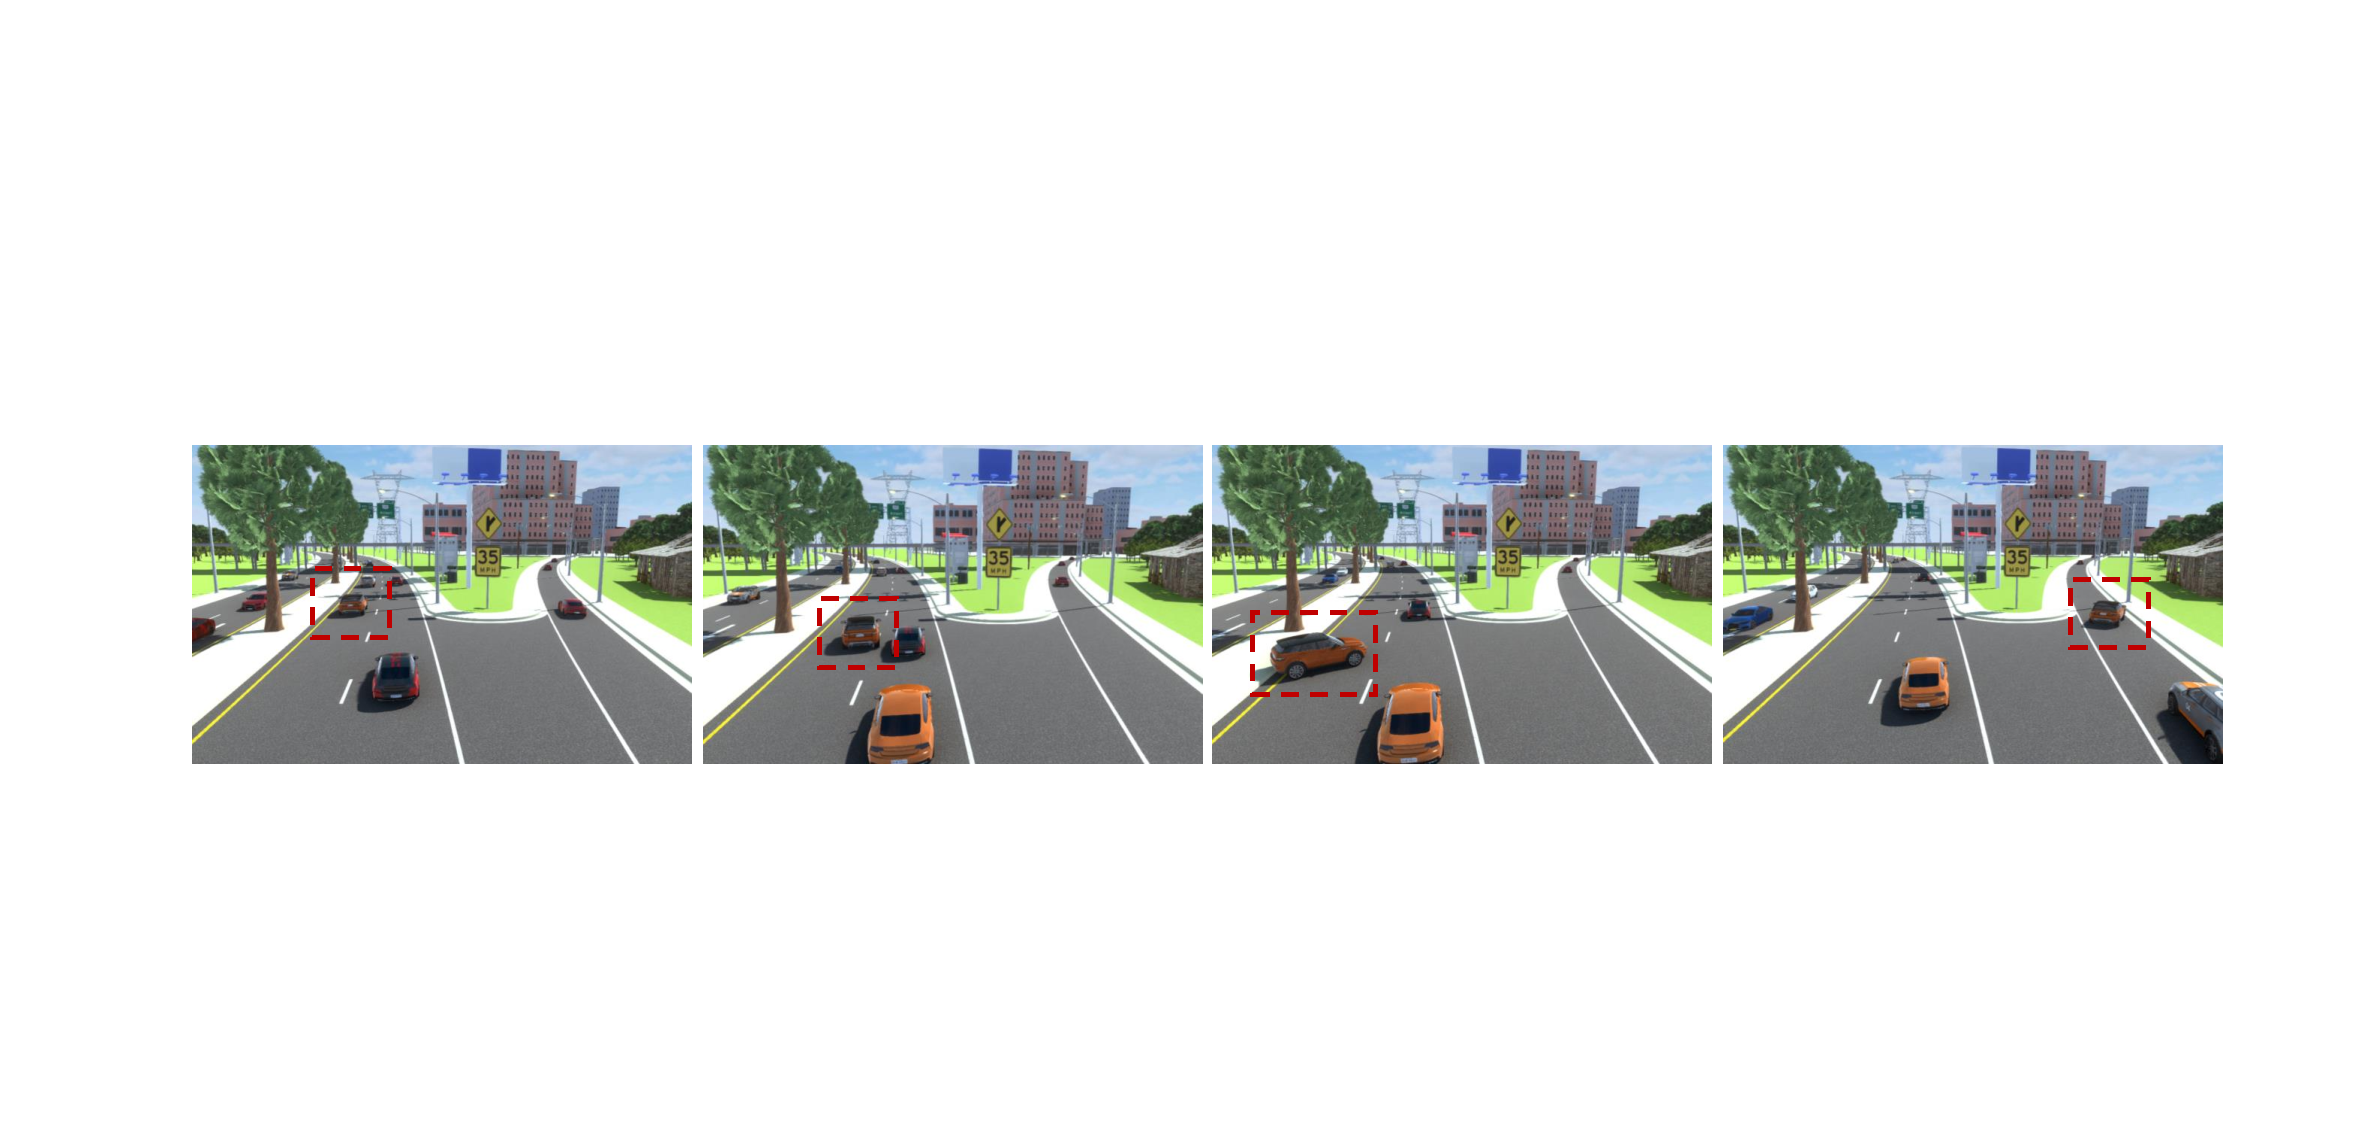
\includegraphics[width=\textwidth]{figure/reversing/teaser v3.pdf}
%\caption[匝道口倒车案例的第三视角示意图]{
%匝道口倒车案例的第三视角示意图,原本车辆在远离匝道的车道上行驶,并已经错过了匝道的出口。使用本方法编辑后,车辆通过倒车回到了匝道出口,并离开主路驶入匝道;而来车则在被编辑车辆完成倒车之前保持静止,等待其通过后方才继续通行。}
\caption[匝道口倒车案例的第三视角示意图]{
匝道口倒车案例的第三视角示意图
}
\label{fig:reversing_teaser}
\end{figure}

本方法主要贡献如下:

\begin{itemize}
    \item 提出了一个新颖的实时交互框架,基于用户偏好引入特定的关键状态,高效地生成具有前向和反向导航的参考路径,又能保证用户交互操作的简便。

    \item 提出了一种基于速度空间采样和能量优化求解约束的个体运动控制方法,满足用户编辑输入的同时,确保车辆在跟驰/非跟驰时都能展现出合理且平滑的运动和交互。

    \item 本方法利用用户的输入驱动车辆的前进和倒车,实现多维度控制的交互式仿真,进一步提高了生成交通场景的多样性和非常规性。
\end{itemize}


\section{方法概述}

图~\ref{fig:reversing_overview}展示了引入倒车行为的交互式交通仿真流程示意图。我们首先介绍了在仿真过程中用于为车辆指定关键状态的交互操作(章节~\ref{section:reversing_keystate}),以及基于关键状态,生成包含前向和反向导航的参考路径所使用的启发式搜索算法(章节~\ref{section:reversing_planning})。为了更新被编辑车辆及其邻车的运动,我们提出了一种基于速度空间采样和能量优化求解约束的交通仿真方法,沿着参考路径来更新车辆状态。所求解的约束包含车辆运动学、自驱动、路径保持和碰撞避免(章节~\ref{section:reversing_dynamics},  ~\ref{section:reversing_optimize})。为了保证车辆在跟驰与非跟驰时都能与邻车合理交互,我们进一步将碰撞避免分解为考虑安全跟随距离的软约束和考虑车辆几何的边界硬约束,同时明细了不同车辆之间的交互优先级(章节~\ref{section:reversing_collisionavoid})。在实验部分,我们展示了使用本方法生成的包含倒车的非常规交通案例(章节~\ref{section:reversing_cases}),并基于对比实验(章节~\ref{section:reversing_comparison})和用户调查(章节~\ref{section:reversing_userstudy})验证了本方法生成的车辆运动的平滑和交互行为的合理。

\begin{figure}[!tbh]
%\setlength{\abovecaptionskip}{-0.1cm} 
%\setlength{\belowcaptionskip}{-0.45cm}
\centering
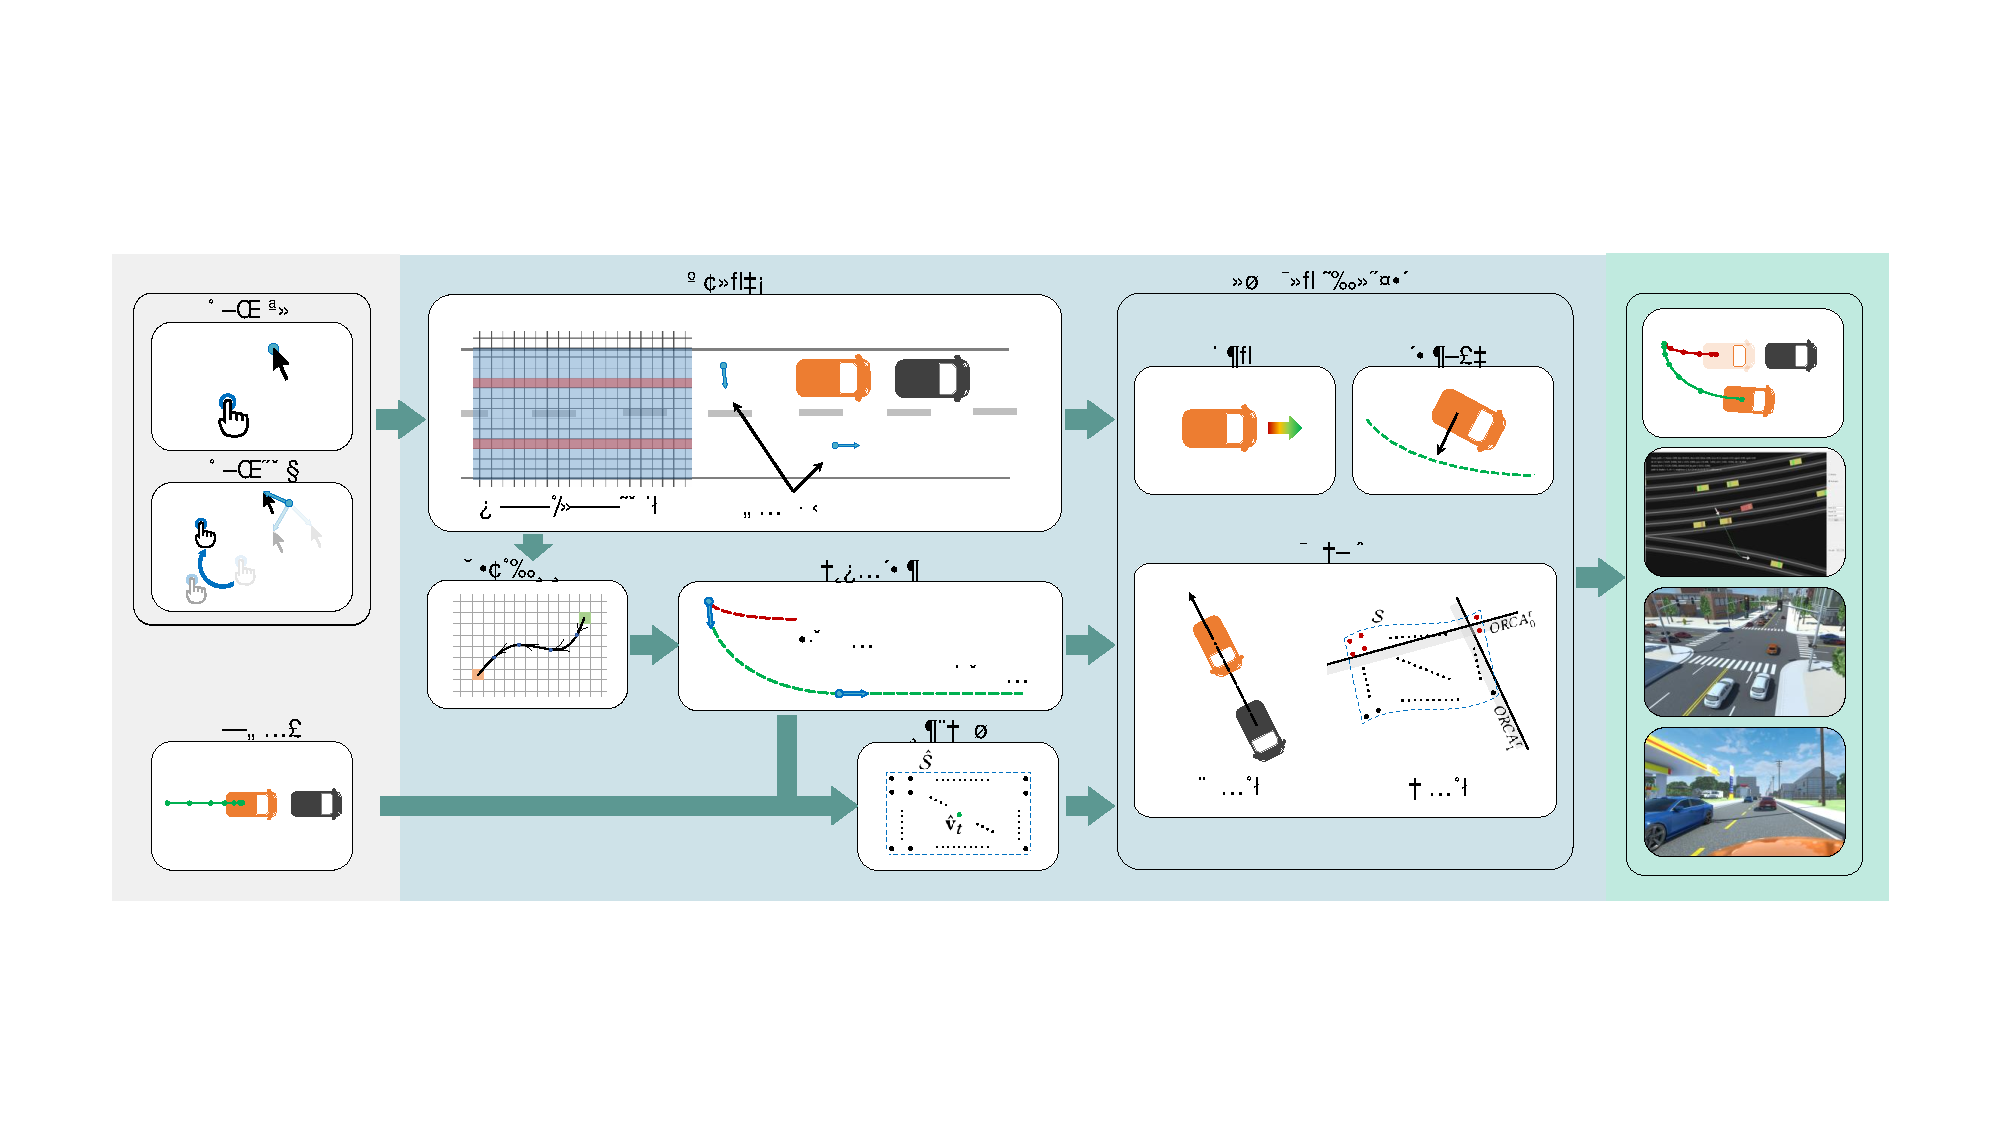
\includegraphics[width=\textwidth]{figure/reversing/overview v3_cn.pdf}
%\caption[引入倒车行为的交互式交通仿真流程示意图]{
%引入倒车行为的交互式交通仿真流程示意图。用户可以使用鼠标为启发式路径搜索点击、拖拽关键状态,生成同时包含前向和反向导航的参考路径。被编辑车辆与邻车通过在速度空间进行采样和能量最优来求解约束以更新运动,包含车辆运动学、自驱动、路径保持、碰撞避免软约束和碰撞避免硬约束等。}
\caption[引入倒车行为的交互式交通仿真流程图]{
引入倒车行为的交互式交通仿真流程图
}
\label{fig:reversing_overview}
\end{figure}


\section{从用户交互到参考路径}
\label{section:reversing_discretize}

与TraEDITS工作一样的是,我们对整个场景进行了预处理,使用相同的流程将整个场景离散化为二维网格,并使用胶囊形状逼近车道几何编码到对应的网格单元中(章节~\ref{section:traedits_discretize})。定义$\mathcal{P}^{l}_{*} = \{\mathcal{P}^{l}_{0}, \mathcal{P}^{l}_{1}, ...\}$表示道路网络拓扑决定的参考路径集合,$\mathcal{P}^{u}_{*} = \{\mathcal{P}^{u}_{0}, \mathcal{P}^{u}_{1}, ...\}$表示用户自定义的参考路径集合,任意可选择的参考路径$\mathcal{P} \in \mathcal{P}^{l}_{*} \cup \mathcal{P}^{u}_{*}$使用三次样条函数进行插值。值得注意的是,由于本工作中的自定义参考路径会同时包含前向和反向导航,因此我们会将一条参考路径中不同导航方向的部分分段进行插值。

\subsection{关键状态的定义与指定}
\label{section:reversing_keystate}

定义$\textbf{p}=(x,y)$, $\hat{\textbf{p}}=(s,d)$, $\textbf{v}=(v^{x}, v^{y})$, $\hat{\textbf{v}}=(v^{s}, v^{d})$和其他拥有相同上标的符号,分别表示在Cartesian坐标系和Frenet坐标系中的位置、速度和其他变量。对于仿真中的一辆车,其在$t$时刻的状态定义为$\textbf{q}_{t} = \{\textbf{p}, \textbf{v},  \hat{\textbf{p}}, \hat{\textbf{v}}, \mathscr{o}, \hat{\textbf{v}}_{e}, \mathcal{P}\} \big|_{t}$,其中$\mathscr{o} \in \mathbb{R}^{1}$表示车辆当前以欧拉角表示的朝向,$\hat{\textbf{v}}_{e} \in \mathbb{R}^2$表示车辆当前预期速度,$\mathcal{P}$表示车辆当前参考路径。现实生活中,车辆在倒车时的朝向和其参考路径的导航方向是相反的。因此用户在生成参考路径的输入中,需要包含区分车辆的朝向和参考路径的导航方向的信息。我们定义用于参考路径生成的关键状态为车辆完整状态的子集,表示为$\Tilde{\textbf{q}} = \{\textbf{p}, \mathscr{o}\} \subsetneqq \textbf{q}$,包含车辆在Cartesian坐标系中的位置和朝向。

\begin{figure}[!tbh]
%\setlength{\abovecaptionskip}{-0.1cm} 
%\setlength{\belowcaptionskip}{-0.45cm}
\centering
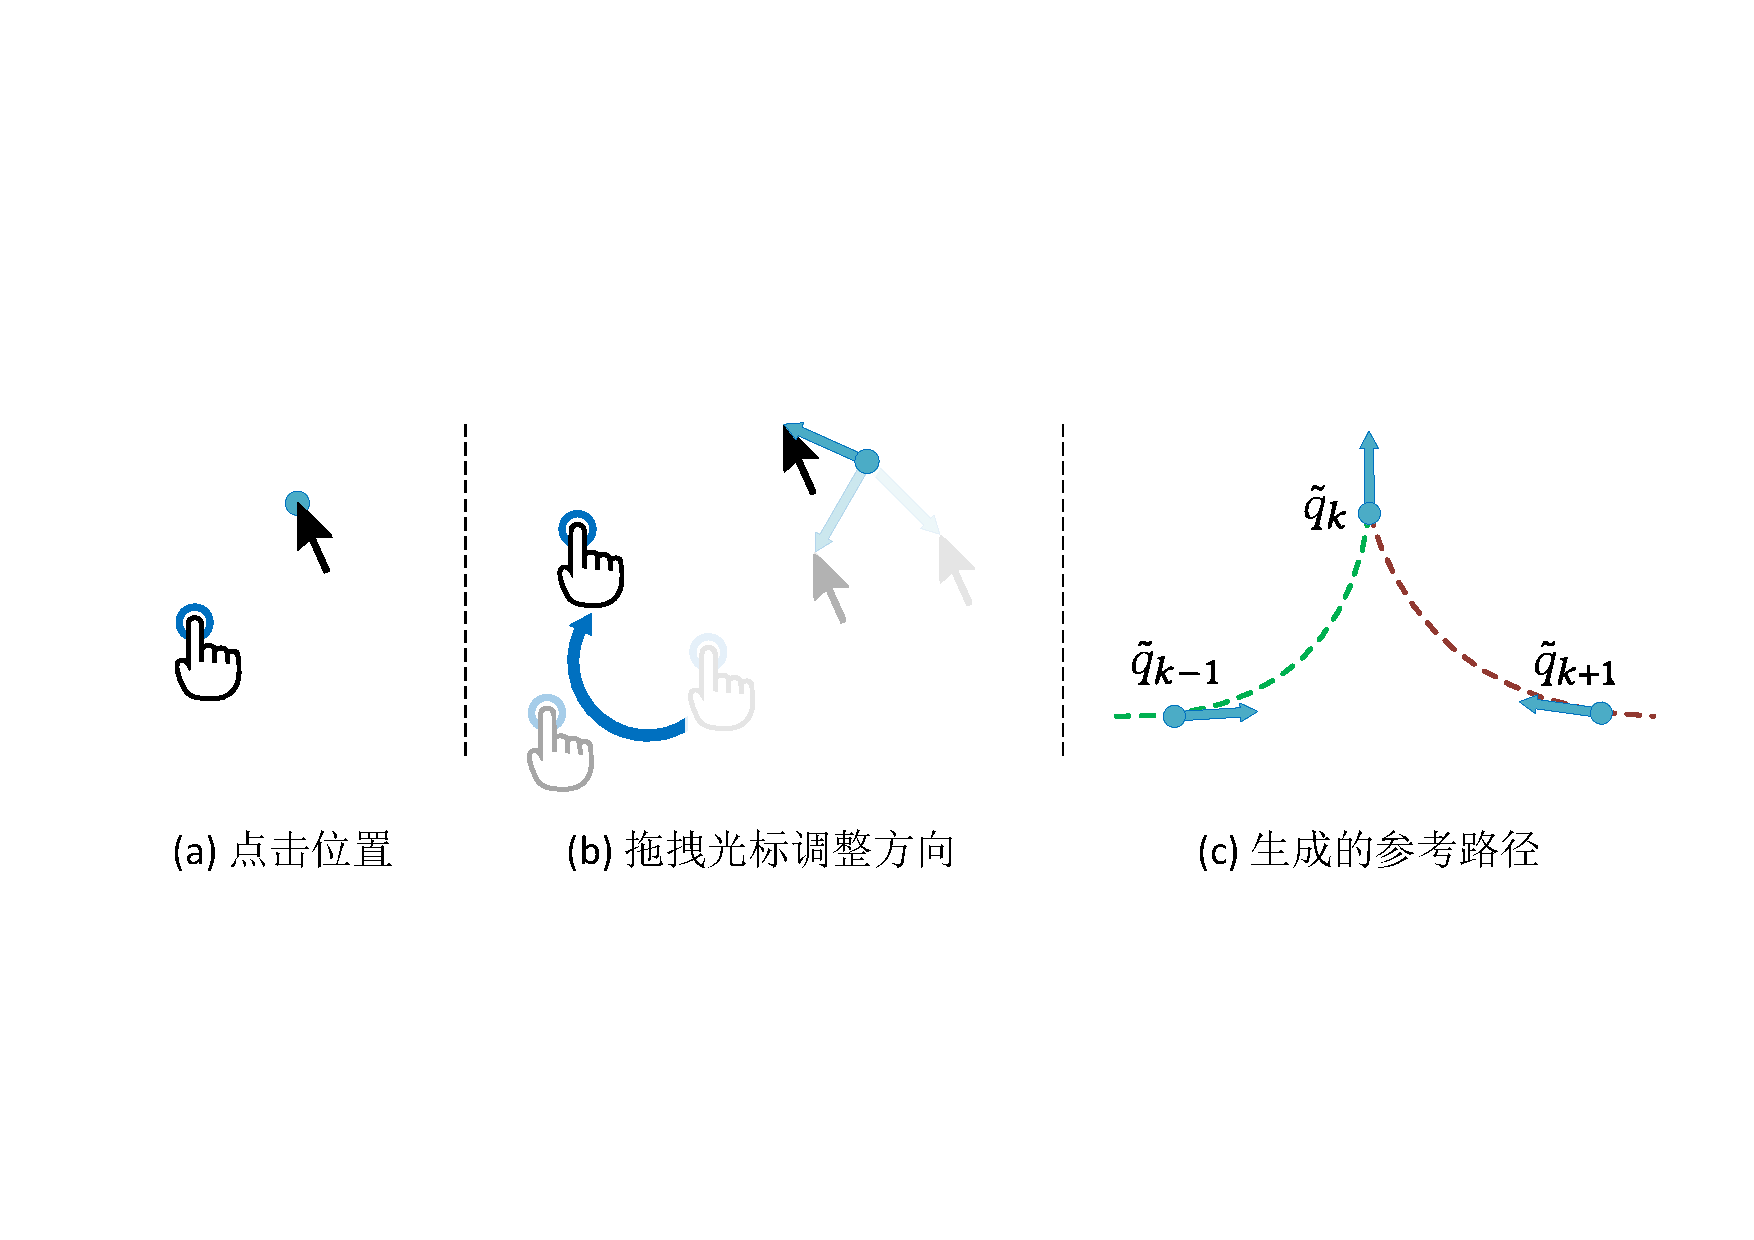
\includegraphics[width=0.9\textwidth]{figure/reversing/cursor v4.pdf}
%\caption[指定关键状态的过程与生成的参考路径]{
%用户指定关键状态的过程与生成参考路径的示意图。(a) 使用光标为关键状态点击位置信息。(b) 保持光标点击状态,为关键状态拖拽相应的朝向。(c) 一部分参考路径示意图,该参考路径由三个有序的关键状态生成,其中绿色段表示前向导航部分,红色段表示反向导航部分。}
\caption[指定关键状态的过程与生成的参考路径]{
指定关键状态的过程与生成的参考路径
}
\label{fig:reversing_keystate}
\end{figure}

用户需要在场景中指定一系列如上的关键状态,用于表示被编辑车辆在未来要依次达到的位置,以及所达到位置时的车辆朝向。图~\ref{fig:reversing_keystate}(a)(b)给出了用户指定一个关键状态的过程示意图,用户首先使用光标为关键状态点击位置,然后保持点击状态拖拽光标来调整关键状态的朝向,最终松开光标完成一个关键状态的指定。图~\ref{fig:reversing_keystate}(c)则展示了一条由三个有序的关键状态生成的参考路径,其中绿色段表示前向导航部分,红色段表示反向导航部分。



\subsection{包含倒车引导的参考路径生成}
\label{section:reversing_planning}

在用户指定了一系列关键状态后,参考路径可以使用启发式搜索算法按照每一对关键状态分段生成,每一对第一个关键状态代表路径搜索的起点,第二个关键状态代表路径搜索的终点。由于需要同时满足位置与朝向的约束,我们使用混合A*算法~\cite{dolgov2008practical}来生成参考路径。相比于传统的路径生成算法只在位置空间中进行规划,混合A*算法充分考虑了车辆前进、后退和转向等行为的运动学模型,把规划过程转移到车辆位置-朝向张成的状态空间中进行,因此能够生成同时包含前向和反向导航的参考路径。混合A*算法的启发式搜索函数定义为:
\begin{equation}
\setlength\abovedisplayskip{10pt}
\setlength\belowdisplayskip{10pt}
\label{eq:reversing_heuristic}
    H(\Tilde{\textbf{q}}) = max\big( RS(\Tilde{\textbf{q}}, \Tilde{\textbf{q}}_{key}, \delta_{0}), H_{0}(\textbf{p}, \textbf{p}_{key}) \big),
    %% reeds_shepp_path.cpp, line34~36
\end{equation}
其中$RS(\Tilde{\textbf{q}}, \Tilde{\textbf{q}}_{key}, \delta_{0})$表示使用Reeds-Shepp曲线模型~\cite{reeds1990optimal}计算得到的启发值,$\delta_{0}$表示一辆车在更新时间步长内的最大转向角,是一个预设常量,而$H_{0}(\textbf{p}, \textbf{p}_{key})$表示使用传统A*算法的启发式函数在位置 $\textbf{p} \in \Tilde{\textbf{q}}$和$\textbf{p}_{key} \in \Tilde{\textbf{q}}_{key}$之间计算得到的启发值。

为了适配我们的实时交互框架,我们对混合A*算法在如下几个方面进行了改进。首先,在进行路径规划之前,为一部分网格单元预计算了启发值$H_{0}(\textbf{p}, \textbf{p}_{key})$并存储在一张查询表内,用于加速表达式~\ref{eq:reversing_heuristic}中每一次传统A*算法启发值的获取。查询表也并非为整张地图的单元网格建立,在A*算法找到一条从起点到终点的最短路径后,我们便停止扩充查询表。只有当后续混合A*算法过程中索引到的网格单元在查询表中无对应数值,才会再次调用A*算法计算。其次,我们在使用混合A*算法规划路径的过程中,会将被编辑车辆的邻车集合中静止的个体视为静态障碍物,让最终生成的参考路径不穿过他们;而对于邻车集合中其他正在运动的个体,我们不在路径规划过程中考虑被编辑车辆与他们的碰撞交互,将基于后续的交通仿真算法进行动态的避障。

得益于结合了Reeds-Shepp曲线模型的混合A*算法,用户实时生成的参考路径$\mathcal{P}^{u}$中,会包含反向导航的部分(如图~\ref{fig:reversing_keystate}(c)所示红色段路径)。由于规划过程考虑了车辆运动学,因此该路径已经足够平滑而无需额外的后处理过程,可直接供仿真中的车辆跟随,记为$\mathcal{P}^{u}_{*} = \mathcal{P}^{u}_{*} \cup \{\mathcal{P}^{u}\}$。



\section{基于速度空间优化的交通仿真算法}



\subsection{基于运动学的车辆状态更新}
\label{section:reversing_dynamics}

由于车辆跟随的参考路径并会同时包含前向和反向导航,因此在一条参考路径中两段相反方向的导航相交的部分会形成一个尖端点(Cusp)。如果仅考虑参考路径的插值函数来计算和更新车辆状态,则车辆在前进和后退切换的时候将会出现严重的动作失真。为了保证车辆在尖端点附近的动作平滑性,我们引入了车辆运动学模型~\cite{laumond2005guidelines}来定义车辆状态的更新过程,表示为一组带约束的能量最优化方程:
\begin{equation}
\label{eq:reversing_dynamics}
\begin{aligned}
    &\hat{\textbf{v}}_{t+1} = \mathop{\arg\min}\limits_{\hat{\textbf{v}}_{r} \in \hat{\mathcal{S}}} \mathcal{E}(\textbf{q}_{t}), \qquad \hat{\textbf{p}}_{t+1} = \hat{\textbf{p}}_{t} + \Delta{t} \cdot \hat{\textbf{v}}_{t+1} , \\
    &\mathscr{o}_{t+1} = \mathscr{o}_{t} + \Delta{t} \cdot \Delta{\mathscr{o}}, \\
    &\Delta{\mathscr{o}} = \omega_{\mathscr{o}} \cdot \frac{|| \hat{\textbf{v}}_{t}||\rm{tan}\delta}{l}, \qquad \delta = \rm{min}(\theta_{t+1} - \theta{t}, \delta_{0}), \\
    &\hat{\textbf{v}}_{e,t} = \mu_{e} \cdot \rm{min}\big( \sqrt{2 |\hat{\textbf{p}}_{c}-\hat{\textbf{p}}_{t}| \odot \hat{\textbf{b}}}, \hat{\textbf{v}}_{e0} \big).
\end{aligned}
\end{equation}
在Frenet坐标系速度空间的一片可行域 $\hat{\mathcal{S}}$中,某一个候选速度$\hat{\textbf{v}}_{r}$表示对于某一辆车而言,其在下一时刻有可能会选择的行驶速度。对于可行域中的所有候选速度,我们使用一个能量函数$\mathcal{E}(\textbf{q}_{t})$去量化地评估其优劣,选择一个能使能量函数值最小的候选速度成为车辆下一时刻的新速度,并根据时间步长$\Delta{t}$更新车辆的Frenet位置坐标。可行域的划分和候选速度的生成将在后续章节中详细介绍。车辆朝向$\Delta{\mathscr{o}}$将根据车辆运动学模型计算出时间步长内的增量后更新得到(如图~\ref{fig:reversing_bicycle}所示),其中$\omega_{\mathscr{o}}$是一个预设的权重系数,$\delta$是车辆当前的转向角,$\delta_{0}$是在时间步长内车辆所能达到的最大转向角,$l$为车辆轴距长度,$\theta_{t}, \theta_{t+1}$为在参考路径的位置点$\hat{\textbf{p}}_{t}, \hat{\textbf{p}}_{t+1}$的切线与水平方向的夹角,也可称为参考路径在该位置点上的方向。车辆的预期速度需要根据即将到来的尖端点$\hat{\textbf{p}}_{c}$位置而实时更新,这是因为车辆在尖端点前后需要进行制动和换挡,保证能在前进和倒车之间平滑切换。$\mu_{e}$是车辆行驶方向的标识符,当其等于$-1$时表示车辆正在倒车,当其等于$1$时表示车辆正在前进,$\odot$表示两个同维向量中对应元素的乘积运算,$\hat{\textbf{b}}$表示车辆在Frenet坐标系中的最大减速度。假如车辆的参考路径后续不存在尖端点,则车辆的预期速度等于预设的最大预期速度$\hat{\textbf{v}}_{e0}$,表示车辆在不受阻的交通环境中希望达到的行驶速度。下一时刻的Cartesian速度$\textbf{v}_{t+1}$和位置$\textbf{p}_{t+1}$可以根据参考路径的样条插值函数计算得到,这里我们不再赘述。

\begin{figure}[!tbh]
%\setlength{\abovecaptionskip}{-0.1cm} 
%\setlength{\belowcaptionskip}{-0.45cm}
\centering
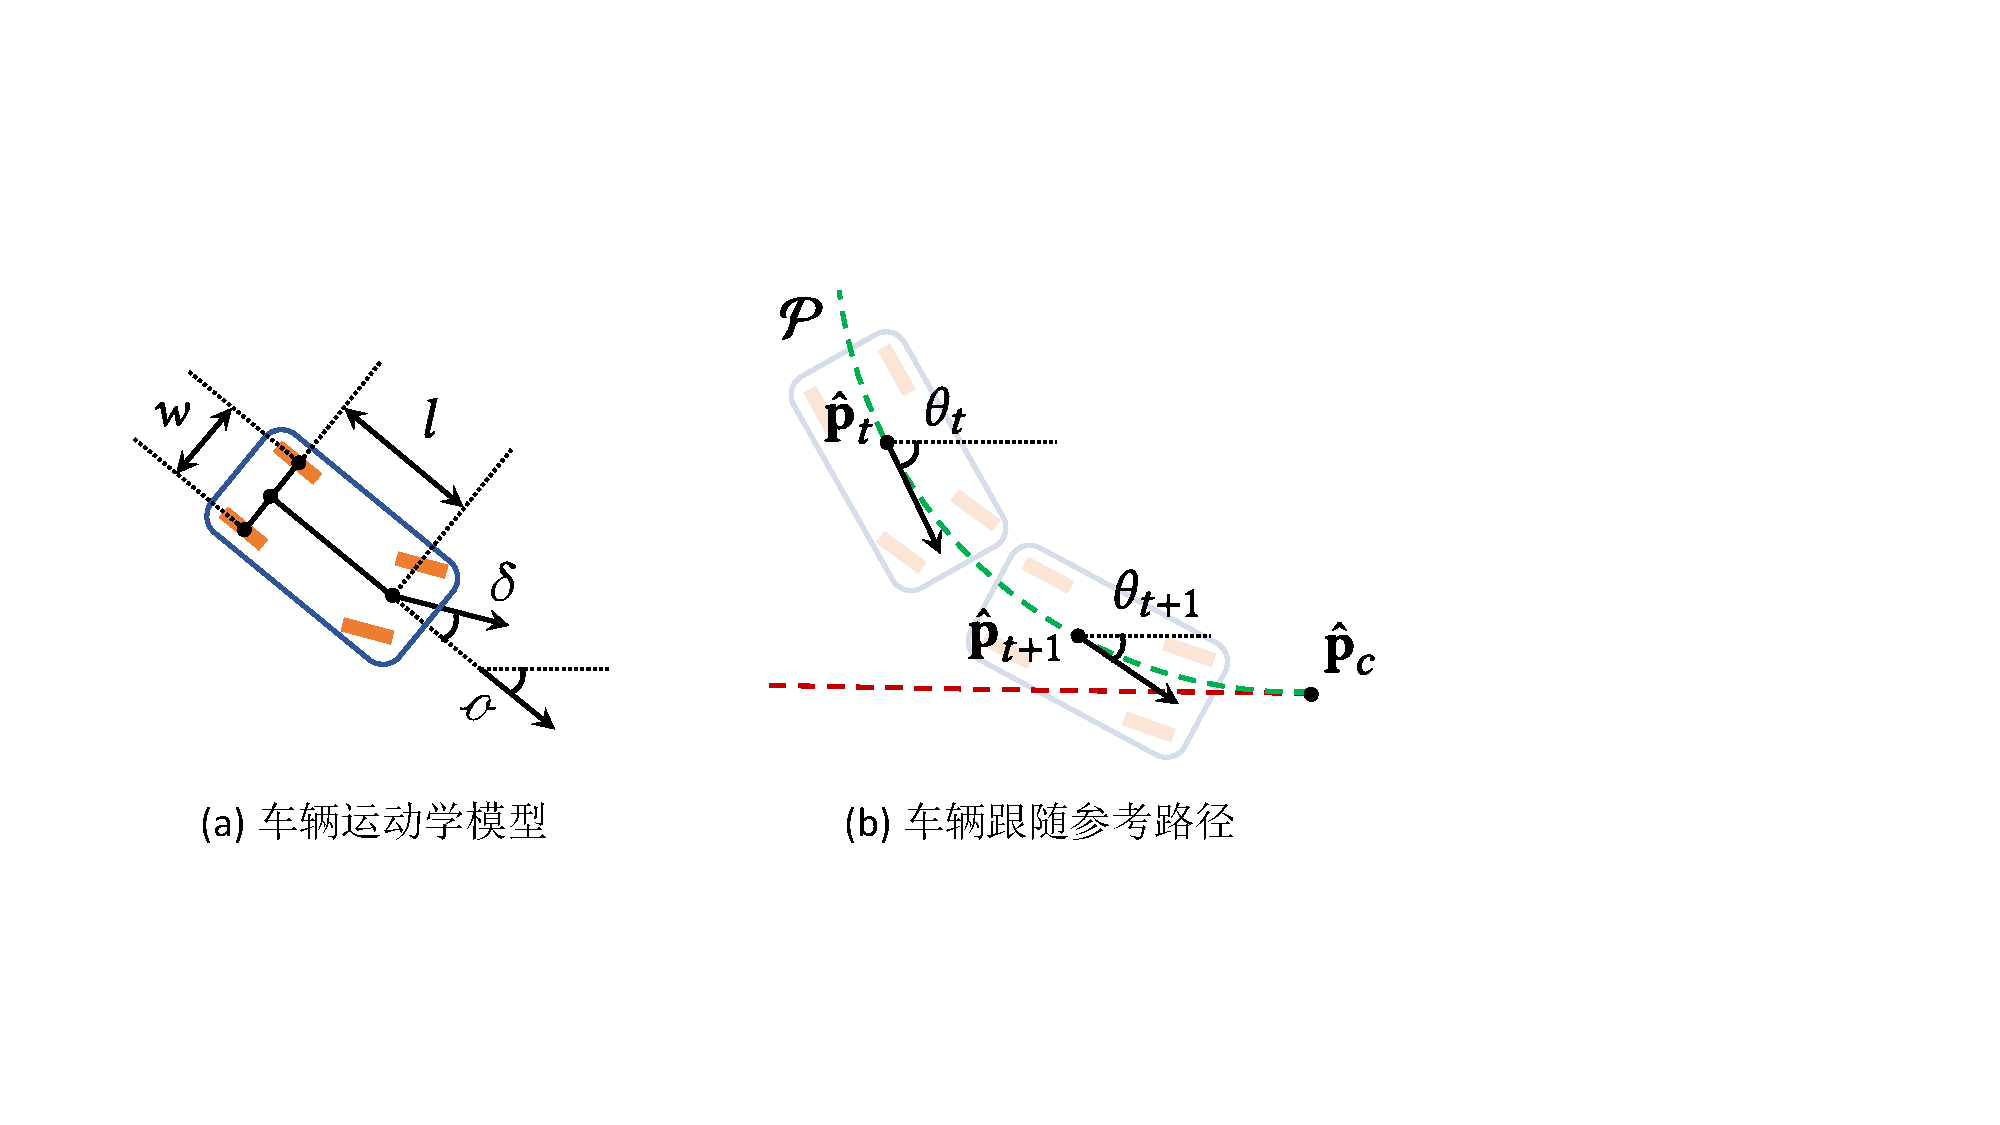
\includegraphics[width=0.85\textwidth]{figure/reversing/bicycle model v4.pdf}
%\caption[车辆运动学模型与参考路径跟随示意图]{
%(a) 仿真部分使用的车辆运动学模型,其中$\mathscr{o}$为朝向,$\delta$为转向角,$l$和$w$分别表示轴距长度和宽度。(b) 一辆车沿着参考路径$\mathcal{P}$行驶,在$t$和$t+1$时刻的状态,其中$\hat{\textbf{p}}_{t}$, $\hat{\textbf{p}}_{t+1}$表示Frenet位置坐标,$\theta_{t}$, $\theta_{t+1}$表示在对应位置点的切线与水平方向的夹角,$\hat{\textbf{p}}_{c}$是一个尖端点的Frenet坐标。}
\caption[车辆运动学模型与参考路径跟随示意图]{
车辆运动学模型与参考路径跟随示意图
}
\label{fig:reversing_bicycle}
\end{figure}



\subsection{速度空间采样与能量最优化仿真}
\label{section:reversing_optimize}

我们通过采样得到计算表达式~\ref{eq:reversing_dynamics}能量最优化的候选速度。对于任意仿真车辆,在Frenet速度空间中,我们基于车辆的当前Frenet速度值、最大加速度和最大减速度,可以确定一个矩形的可行域$\hat{\mathcal{S}}$,该可行域代表车辆受加速度限制在下一时刻所能到达的速度范围。给定采样步长,我们在该可行域范围内均匀采样一系列候选速度$\hat{\textbf{v}}_{r} \in \hat{\mathcal{S}}$,用于能量最优化的计算。图~\ref{fig:reversing_velspace}(a)展示的是根据一辆正向行驶的车辆的当前状态,在Frenet速度空间中划分的可行域和采样得到的候选速度。假如是一辆倒车中的车辆,其可行域应当落在纵向速度分量$v^{s}$坐标轴的负轴范围内。图~\ref{fig:reversing_velspace}(b)为Frenet坐标系中的采样候选速度转换到Cartesian坐标系中的结果示意图,我们可以通过参考路径的三次样条插值函数计算得到$\textbf{v}_{r} \in \mathcal{S}$。此外,对于Frenet速度空间中的可行域,我们还会额外使用车辆在道路上的最大行驶速度来限制其范围,防止其超速。


\begin{figure}[!tbh]
%\setlength{\abovecaptionskip}{-0.1cm} 
%\setlength{\belowcaptionskip}{-0.45cm}
\centering
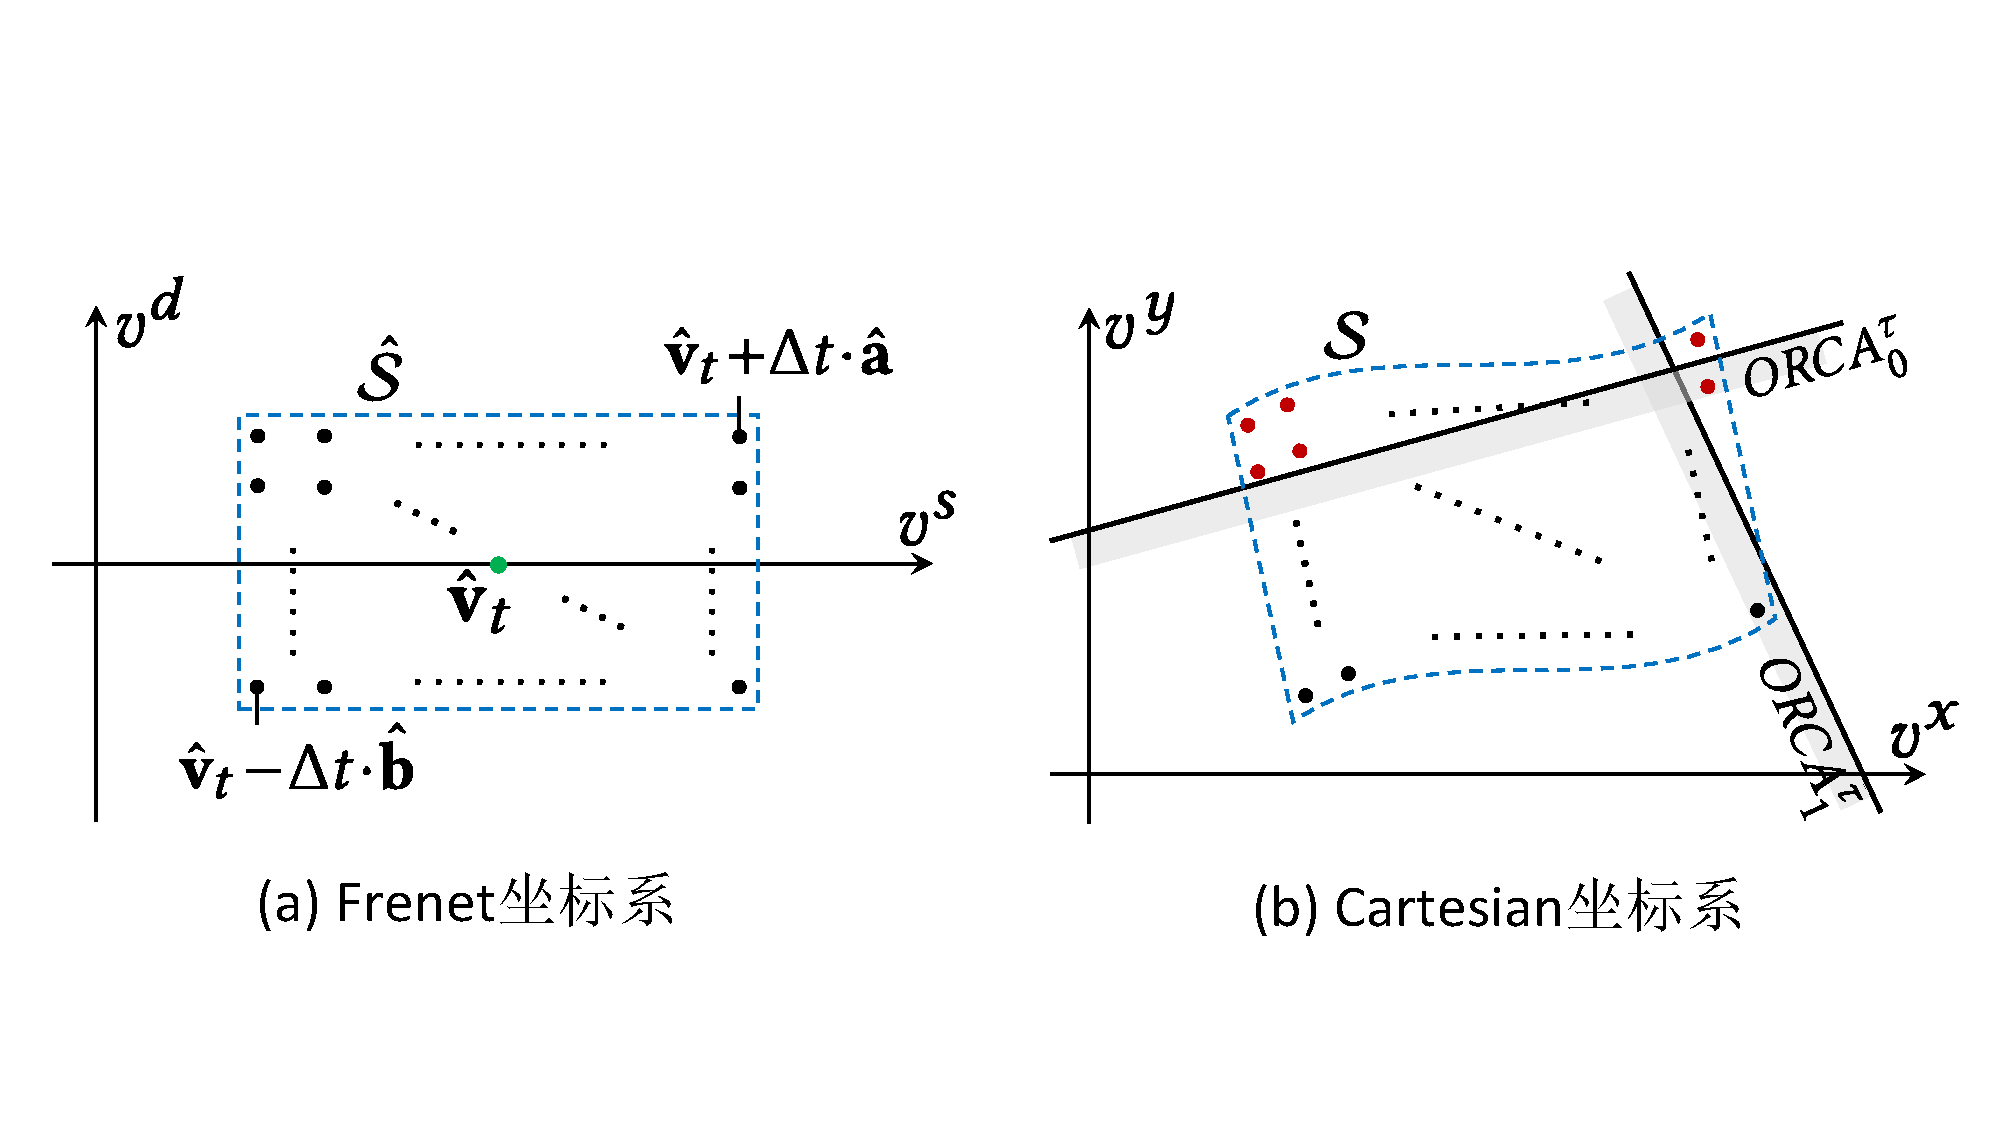
\includegraphics[width=0.85\textwidth]{figure/reversing/velocity space v2.pdf}
%\caption[各坐标系中速度空间可行域的划分与采样]{
%(a) 在Frenet坐标系中,由一辆前向行驶的车辆的当前速度、最大加速度与最大减速度决定的候选速度采样可行域$\hat{\mathcal{S}}$。(b) 在Cartesian坐标系中,候选速度采样可行域$\mathcal{S}$与基于ORCA算法得到的碰撞避免边界硬约束。}
\caption[不同坐标系中速度空间可行域的划分与采样]{
不同坐标系中速度空间可行域的划分与采样
}
\label{fig:reversing_velspace}
\end{figure}

对于每一个候选速度,我们使用关于车辆当前状态$\textbf{q}_{t}$的能量函数$\mathcal{E}$来计算一个能量值。我们在能量函数中考虑了三个强烈影响车辆运动的因素,即自驱动,路径保持和碰撞避免:
\begin{equation}
\setlength\abovedisplayskip{10pt}
\setlength\belowdisplayskip{10pt}
\label{eq:reversing_totenergy}
    \mathcal{E} = \omega_{e}\mathcal{E}_{e} + \omega_{k}\mathcal{E}_{k} + \omega_{c}\mathcal{E}_{c},
\end{equation}
其中$\mathcal{E}_{e}$是自驱动能量项,用于使车辆保持预期速度行驶;$\mathcal{E}_{k}$是路径保持能量项,用于使车辆保持沿参考路径行驶;$\mathcal{E}_{c}$是碰撞避免能量项,用于使车辆避免与邻车发生碰撞。$\omega_{e}, \omega_{k}, \omega_{c}$分别是上述三个能量项的求和权重。

\textbf{自驱动项:}自启动项定义为:
\begin{equation}
\setlength\abovedisplayskip{10pt}
\setlength\belowdisplayskip{10pt}
\label{eq:reversing_selfmotive}
    \mathcal{E}_{e} = e^{|| \hat{\textbf{v}}_{r} - \hat{\textbf{v}}_{e,t} ||},
\end{equation}
其中$\hat{\textbf{v}}_{e,t}$是车辆当前的预期速度。

\textbf{路径保持项:}路径保持项定义为:
\begin{equation}
\setlength\abovedisplayskip{10pt}
\setlength\belowdisplayskip{10pt}
\label{eq:reversing_pathkeep}
    \mathcal{E}_{k} = 
    \left\{
        \begin{array}{lr}
        e^{|\Delta{t} \cdot v^{d}_{r}|}, & | d_{t}| \geq \frac{1}{2}w \\
        0, & \rm{otherwise}
        \end{array}, 
    \right.
\end{equation}
其中$v^{d}_{r} \in \hat{\textbf{v}}_{r}$表示候选速度的横向分量,$d_{t} \in \hat{\textbf{p}}_t$表示车辆Frenet位置坐标的横向分量,$w$是轴距宽度。如上式所示,为了防止车辆在参考路径附近来回振荡,路径保持项只有在车辆与参考路径的距离超过给定阈值时才生效。

\textbf{碰撞避免项:}对于一辆车和一个给定的搜索范围,我们寻找其在时刻$t$下的邻车集合$\mathcal{N}_t$,则碰撞避免项由两部分组成:
\begin{equation}
\setlength\abovedisplayskip{10pt}
\setlength\belowdisplayskip{10pt}
\label{eq:reversing_totcollision}
    %\mathcal{E}_{c} = \mathcal{E}^{s}_{c}(\textbf{q}_{t}) + \mathcal{E}^{h}_{c}(\textbf{q}_{t}),
    \mathcal{E}_{c} = \mathcal{E}^{s}_{c} + \sum\nolimits_{j \in \mathcal{N}_{t}} \mathcal{E}^{h}_{c, j},
\end{equation}
其中第一项为考虑车辆安全跟车距离的软约束,第二项为考虑车辆几何信息的边界硬约束,二者按规定发生作用才能保证车辆在展现跟驰行为和非跟驰行为时都能与邻车正确地交互。


\subsection{多约束碰撞避免与车辆交互规则}
\label{section:reversing_collisionavoid}

\textbf{碰撞避免软约束:}表达式~\ref{eq:reversing_totcollision}中的第一项用于保证车辆在跟驰运动时,随着与前车的距离变小而逐渐减速,最终要停止在一个安全的距离之外。其定义为:
\begin{equation}
\setlength\abovedisplayskip{10pt}
\setlength\belowdisplayskip{10pt}
\label{eq:reversing_softcollision}
    \mathcal{E}^{s}_{c} = 
    \dfrac{
    ||\textbf{v}_{r}||T_{0} + %\frac{||\textbf{v}|| ||\textbf{v} - \textbf{v}_{leader}||}{2 \sqrt{\hat{\textbf{a}} \hat{\textbf{b}}}}
    \tfrac{1}{2} ||\textbf{v}_{r}|| ||\textbf{v}_{l,t}-\textbf{v}_{r}|| / \sqrt{\hat{\textbf{a}} \hat{\textbf{b}}}
    }{
    (1+ || \textbf{p}_{l,t} - \textbf{p}_{r} || / s_{0} )^2
    },
\end{equation}
其中$s_{0}, T_{0}$分别表示给定的车辆安全跟随距离和制动反应时间,$\textbf{p}_{r}$表示如果车辆以候选速度$\hat{\textbf{v}}_{r}$行驶下一时刻的预期Cartesian位置坐标,$\textbf{v}_{l,t}, \textbf{p}_{l,t}$则分别表示前车$l = \exists j \in \mathcal{N}_{t}$的Cartesian速度和位置坐标。假如当前车辆前方范围内没有车辆,则该项不会生效。


\textbf{碰撞避免硬约束:}表达式~\ref{eq:reversing_totcollision}中的第二项是一项考虑了所有在集合中的邻车$j \in \mathcal{N}_{t}$的几何计算得到的边界约束$\mathcal{E}^{h}_{c}$,用于避免车辆在非跟驰运动时由于安全跟车距离失效而发生的碰撞或剐蹭。举例来说,当一辆车同时被前车和后车阻挡,驾驶员可能会通过前后挪车来获取一个更大的转向角,然后从侧方驶离该位置,而此运动过程中车辆与邻车的距离将会远小于安全跟车距离,即安全跟车距离失效。如图~\ref{fig:reversing_velspace}(b)所示,对于任意邻车$j \in \mathcal{N}_{t}$我们为其计算ORCA直线~\cite{van2011reciprocal},每一个ORCA直线将速度空间分为两个半平面,一半包含了会与对应邻车$j$发生碰撞的速度,另一半则是不会与$j$发生碰撞的速度。因此,速度空间中的可行域$\mathcal{S}$会被一系列ORCA直线划分为更小的不规则区域,进一步将会发生碰撞的候选速度排除在外。该过程定义为:
\begin{equation}
\setlength\abovedisplayskip{10pt}
\setlength\belowdisplayskip{10pt}
\label{eq:reversing_hardcollision}
\begin{aligned}
    & \mathcal{E}^{h}_{c,j} = \left\{
        \begin{array}{lr}
        0, & \textbf{v}_{r} \in ORCA^{\tau}_{j} = \{ \textbf{v} \big| \left( \textbf{v} - (\textbf{v}_{t} + \textbf{u}) \cdot \textbf{n} \right) \geq 0 \} \\
        \mathcal{E}_{0}, & \rm{otherwise}
        \end{array}, 
    \right. %\\
    %& c = \frac{1}{s_0},
\end{aligned}
\end{equation}
其中$\mathcal{E}_{0}$是一个很大的预设值,用于惩罚可行域内但落在ORCA直线范围外的候选速度(如图~\ref{fig:reversing_velspace}(b)中的红色圆点所示),$\tau$是计算ORCA直线对应的VO所用的时间范围,$\textbf{v}_{t}$是当前车辆的Cartesian速度,$\textbf{u}$表示在时间范围$\tau$内车辆与邻车$j$若恰好发生碰撞需要的相对速度变化量,$\textbf{n}$则表示指向VO外侧的单位向量,其等于归一化后的向量$\textbf{u}$或是相反向量。需要注意的是,我们计算VO所使用的时间范围$\tau$也是动态改变的,其等于当前车辆完全停止所需的时间和制动反应时间之中更大的一方,即:
\begin{equation}
\setlength\abovedisplayskip{10pt}
\setlength\belowdisplayskip{10pt}
\label{eq:reversing_tau}
    \tau = \rm{max}(T_{0}, \frac{|| \hat{\textbf{v}}_{t} ||}{|| \hat{\textbf{b}} ||}).
    %\tau = \rm{max}(T_{0}, || \hat{\textbf{v}}_{t} ||/|| \hat{\textbf{b}} ||).
\end{equation}
由于VO和ORCA是机器人领域求解无碰撞运动的经典算法,因此具体实现细节可参考绪论部分的内容或相关工作~\cite{van2008reciprocal, van2011reciprocal},在此我们不做赘述。

\begin{figure}[t]
%\setlength{\abovecaptionskip}{-0.1cm} 
%\setlength{\belowcaptionskip}{-0.45cm}
\centering
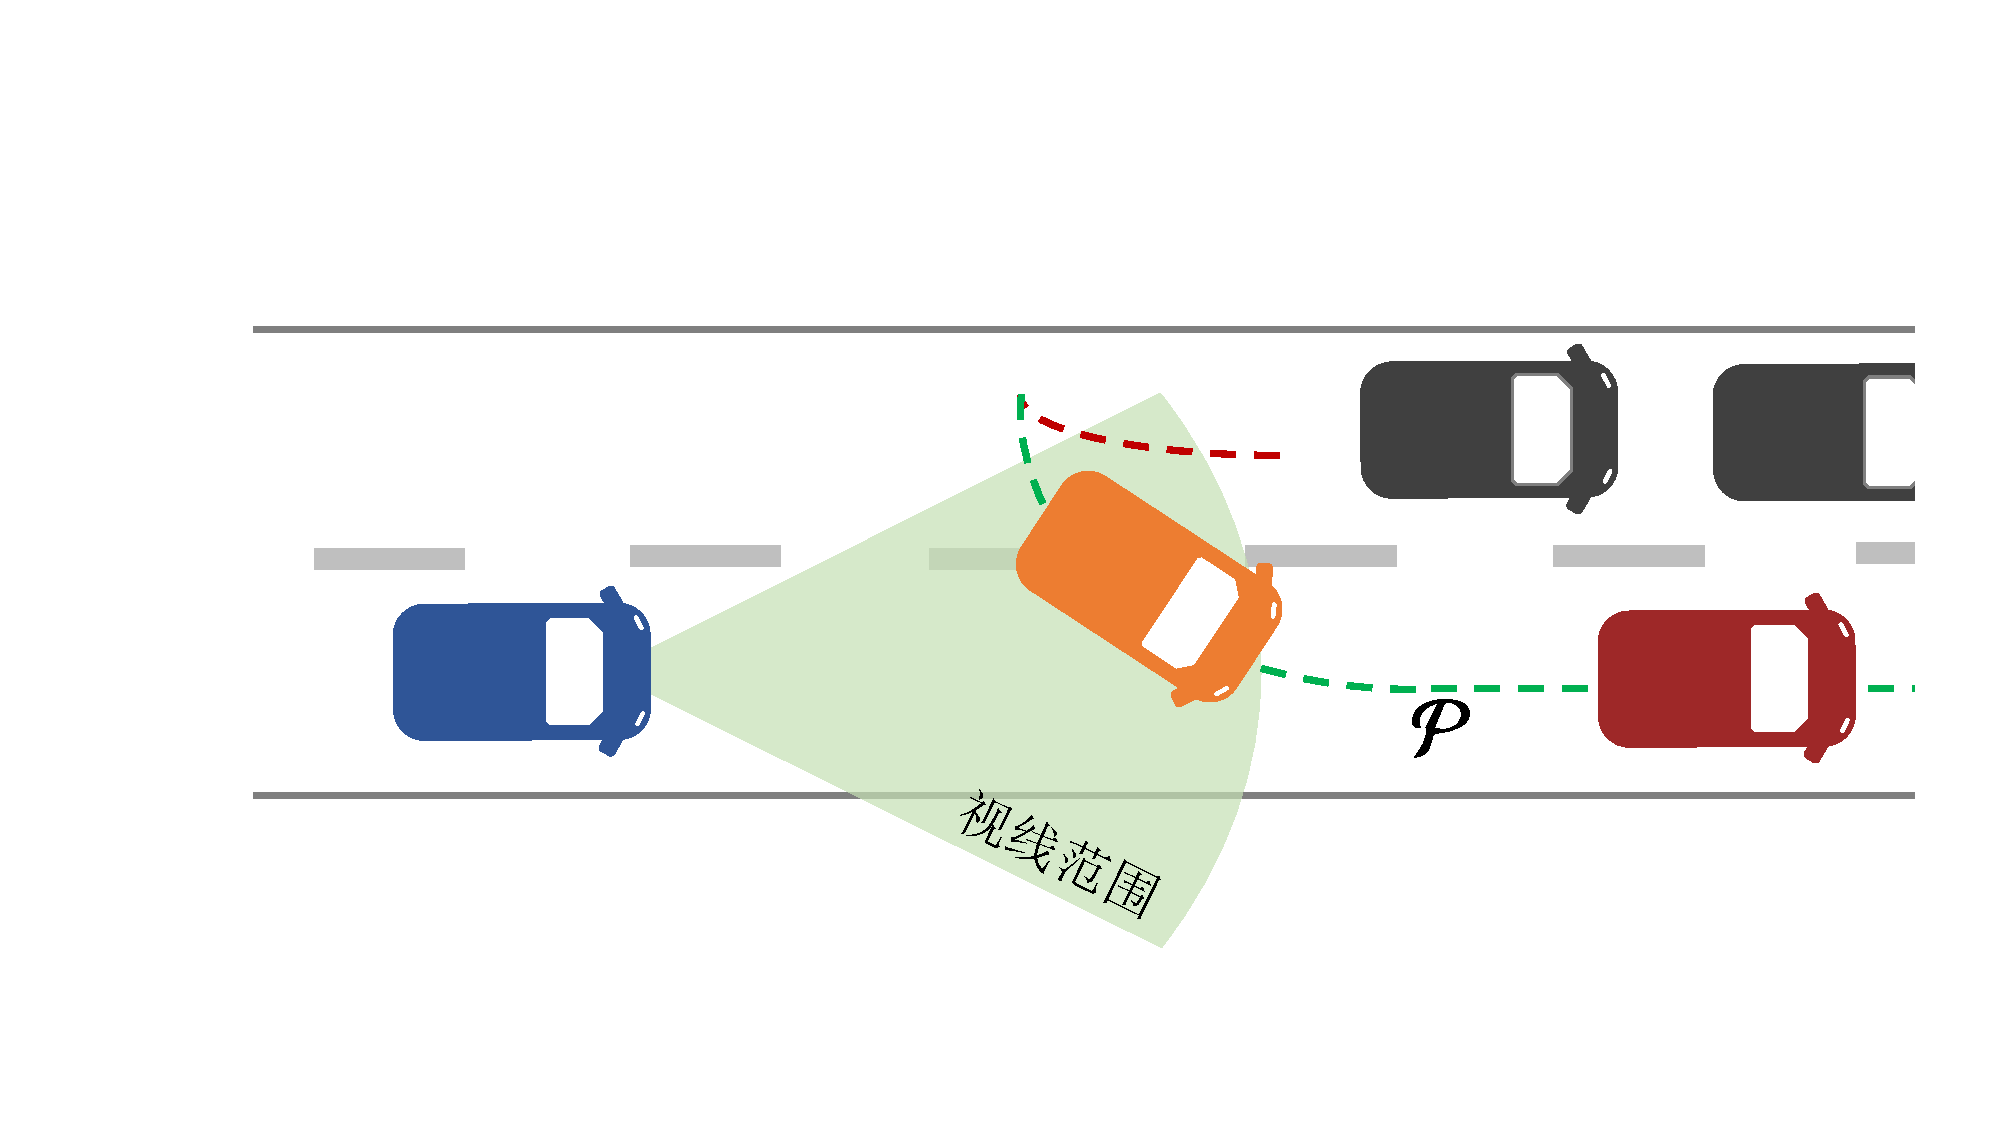
\includegraphics[width=0.65\textwidth]{figure/reversing/on road v2_cn.pdf}
%\caption[非跟驰车辆与跟驰车辆交互示意图]{
%在道路上,一辆非跟驰运动中的车辆(橙色)沿着其参考路径$\mathcal{P}$行驶。该非跟驰车辆处于跟驰车辆(蓝色)的视线范围内,同时该非跟驰车辆的参考路径穿过另一辆跟驰车辆(红色),我们分别对这些交互行为的优先级进行了定义。}
\caption[非跟驰车辆与跟驰车辆交互场景]{
非跟驰车辆与跟驰车辆交互场景
}
\label{fig:reversing_onroad}
\end{figure}


\begin{table}[b]
%\setlength{\abovecaptionskip}{-0.001cm}
\setlength{\belowcaptionskip}{0.4cm}
\centering
%\caption[不同运动类型车辆之间的交互规则]{不同运动类型车辆之间的交互规则。(a) 开启碰撞避免软约束$\mathcal{E}^{s}_{c}$使安全跟随距离生效。(b) 若邻车持续存在于车辆的视线范围内,强行使车辆制动直至停止。(c) 开启碰撞避免硬约束$\mathcal{E}^{h}_{c}$。(d) 若车辆的参考路径穿过邻车,开启碰撞避免软约束$\mathcal{E}^{s}_{c}$使安全跟随距离生效。}
\caption[不同运动类型车辆之间的交互规则]{
不同运动类型车辆之间的交互规则
}
\label{tab:reversing_rules}
\renewcommand\arraystretch{1.7}
\begin{tabular}{@{}clcc@{}}
\toprule
\multicolumn{2}{c}{\multirow{2}{*}{$\qquad$车辆运动类型$\qquad$}} & \multicolumn{2}{c}{$\qquad$邻车运动类型$\qquad$} \\ \cmidrule(l){3-4} 
\multicolumn{2}{c}{}                                     & 跟驰     & 非跟驰    \\ \midrule
\multicolumn{2}{c}{跟驰}                        & 开启碰撞避免软约束               & 强行制动至停止                  \\
\multicolumn{2}{c}{非跟驰}                    & 开启碰撞避免软、硬约束               & 开启碰撞避免软、硬约束                  \\ \bottomrule
\end{tabular}
\end{table}


\textbf{车辆交互规则:}经过用户编辑后,交通场景中可能会同时存在非跟驰运动的车辆和跟驰运动的车辆,这使得车辆之间的交互变得更加复杂。为了避免不同运动类型的车辆在交互过程中互不相让而引起交通瘫痪,我们设计了一系列规则以明细各个车辆之间交互的优先级,如表~\ref{tab:reversing_rules}所示。我们将跟随的参考路径中具有后向导航的车辆归类为非跟驰车辆,将其他车辆归类为跟驰车辆,车辆类型会根据参考路径的变化而动态变化。对于一辆跟驰运动的车辆,如果其邻车也都是跟驰运动,碰撞避免将只生效软约束$\mathcal{E}^{s}_{c}$,使其更注重于与前车的跟随行为;如果其视线范围内持续存在一辆非跟驰运动的邻车(如图~\ref{fig:reversing_onroad}所示的蓝色车辆),该车辆会被强行停止,直到该非跟驰车辆驶离实现范围或结束非跟驰运动,这是因为一辆在道路上倒车的车辆会引起别人更多的关注和戒备心。对于一辆非跟驰运动的车辆,碰撞避免中的边界硬约束$\mathcal{E}^{h}_{c}$将会持续生效,而软约束只有在该车的参考路径未来穿过某一辆邻车时才会生效(如图~\ref{fig:reversing_onroad}所示的红色车辆)。换句话说,一辆非跟驰车辆在其参考路径无法保证完全避免碰撞的情况下,仍需要与阻碍在其行驶路径上其他车辆保持安全跟随距离。



\section{实验结果}

\subsection{实现细节}

后续实验所用的设备为一台台式电脑,配置了8核的3.60GHz Intel(R) Xeon(R) W-2123处理器以及32GB的内存。我们的核心代码基于C++实现,用户交互编辑的图形化界面使用Qt构建,生成的交互式仿真轨迹导出后在Unity3D中进行可视化,以获得更真实的交通场景结果,如图~\ref{fig:reversing_gui}所示。

\begin{figure}[!tbh]
%\setlength{\abovecaptionskip}{-0.1cm} 
%\setlength{\belowcaptionskip}{-0.45cm}
\centering
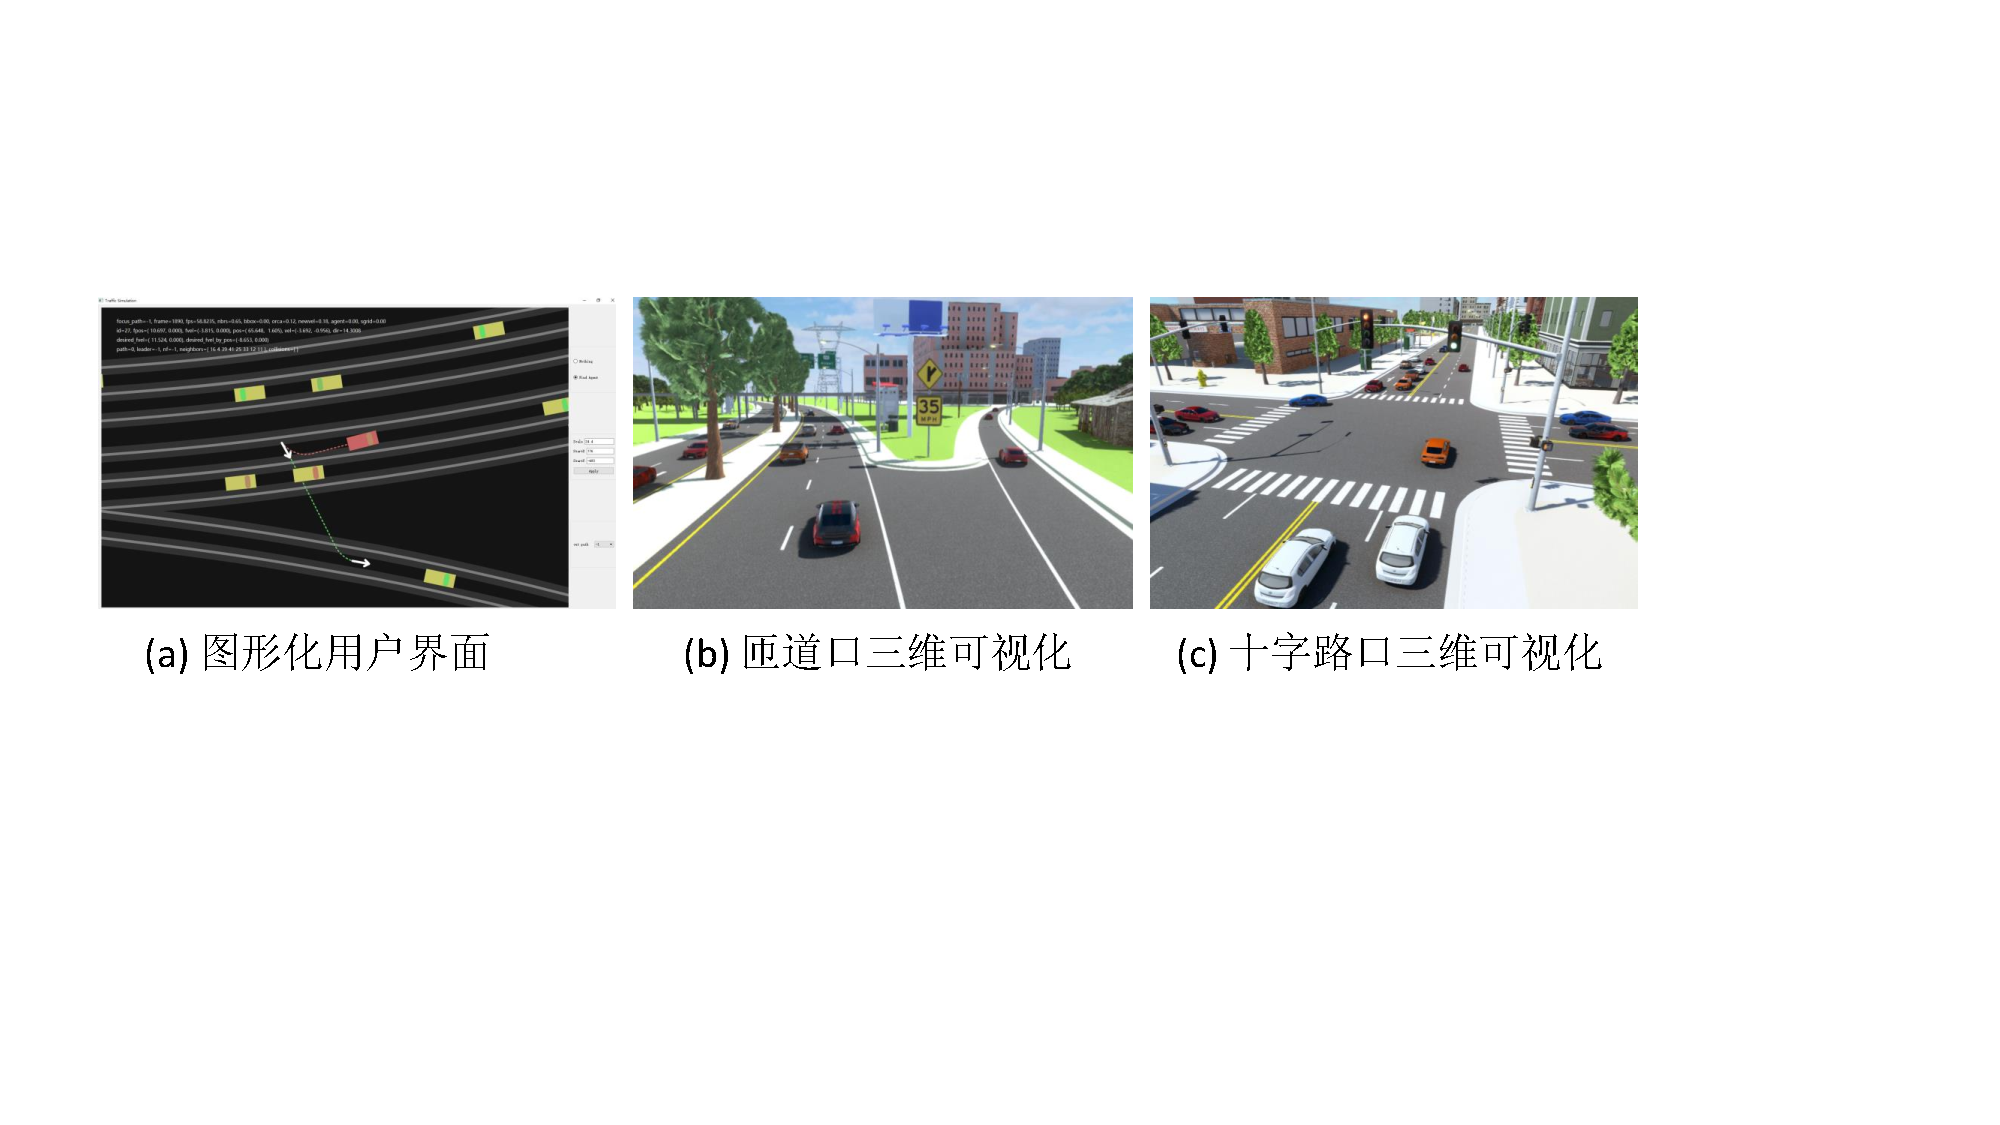
\includegraphics[width=0.96\textwidth]{figure/reversing/gui v3.pdf}
%\caption[图形化用户界面与包含非跟驰行为的交通场景]{
%(a) 交互式轨迹编辑的图形化用户界面,使用Qt搭建。(b,c) 实验中所用的场景在Unity3D中进行可视化。}
\caption[图形用户界面与三维可视化结果]{
图形用户界面与三维可视化结果
}
\label{fig:reversing_gui}
\end{figure}

\begin{table}[!tbh]
%\setlength{\abovecaptionskip}{-0.01cm}
\setlength{\belowcaptionskip}{0.4cm}
\centering
\caption[实验中所用到的一些重要参数的取值]{实验中所用到的一些重要参数的取值}
\label{tab:reversing_parameters}
\renewcommand\arraystretch{1.4}
\begin{tabular}{@{}cccc@{}}
\toprule
参数                            & 取值                & 单位      & 描述                                                                                                 \\ \midrule
$\delta_{0}$                         & $10.0$               & 弧度     & 时间步长内车辆的最大转向角        \\
$\omega_{\mathscr{o}}$                & 5.0                  & $-$       & 表达式~\ref{eq:reversing_dynamics}中的转向角更新系数                        \\
$\hat{\textbf{a}}$                   & $(3.5 \pm 0.5, 1.0)$ & $m/s^{2}$ & Frenet坐标系中车辆的最大加速度                                     \\
$\hat{\textbf{b}}$                   & $(6.0 \pm 1.0, 1.0)$ & $m/s^{2}$ & Frenet坐标系中车辆的最大减速度                                           \\
$l, w$                               & $3.6, 1.7$           & $m$       & 车辆轴距的长度和宽度                                                     \\
$\omega_{e}, \omega_{k}, \omega_{c}$ & $1.0, 10.0, 8.0$     & $-$       & 表达式~\ref{eq:reversing_totenergy}中能量函数的求和权重                   \\
$T_{0}$                              & $1.0 \pm 0.5$        & $s$       & 车辆的制动反应时间                                                                  \\
$S_{0}$                              & $4.0 \pm 1.0$        & $m$       & 车辆与前车的安全跟随距离                                      \\
$\mathcal{E}_{0}$                    & 1E5                  & $-$       & 表达式~\ref{eq:reversing_hardcollision}中落在边界约束外的惩罚项 \\ \bottomrule
\end{tabular}
\end{table}


实验中所用的场景为使用Mathworks的产品RoadRunner手工生成。我们从生成好的场景中导出道路信息为XML文件,并进一步使用SUMO NetEdits后处理生成道路网络的拓扑关系(即入车道,出车道和邻车道),最终导入到程序中生成初始化的道路网络拓扑决定的参考路径集合$\mathcal{P}^{l}_{*}$;而生成好的场景中的三维物体可以直接导出成FBX文件,并导入到Unity3D中使用。章节~\ref{section:reversing_discretize}中提及的场景离散化所使用的分辨率为$0.5m \times 0.5m$,章节~\ref{section:reversing_optimize}中提及的速度空间采样步长为$7 \times 7$,即包含车辆当前速度在内,最终可行域内会采样出50个候选速度,每一辆车的邻车集合$\mathcal{N}_{t}$搜索范围为$100 \times 100$个单元网格。其他的一些重要参数取值如表~\ref{tab:reversing_parameters}所示,这些参数均在配置文件中提前定义,并在程序运行时被动态加载。


\subsection{倒车行为生成案例}
\label{section:reversing_cases}



我们在不同的场景中设计了一些案例,用于展示使用本方法交互式仿真生成的包含非跟驰运动的交通场景,这些案例在以往的交通仿真方法中难以实现。

\begin{figure}[!tbh]
%\setlength{\abovecaptionskip}{-0.1cm} 
%\setlength{\belowcaptionskip}{-0.45cm}
\centering
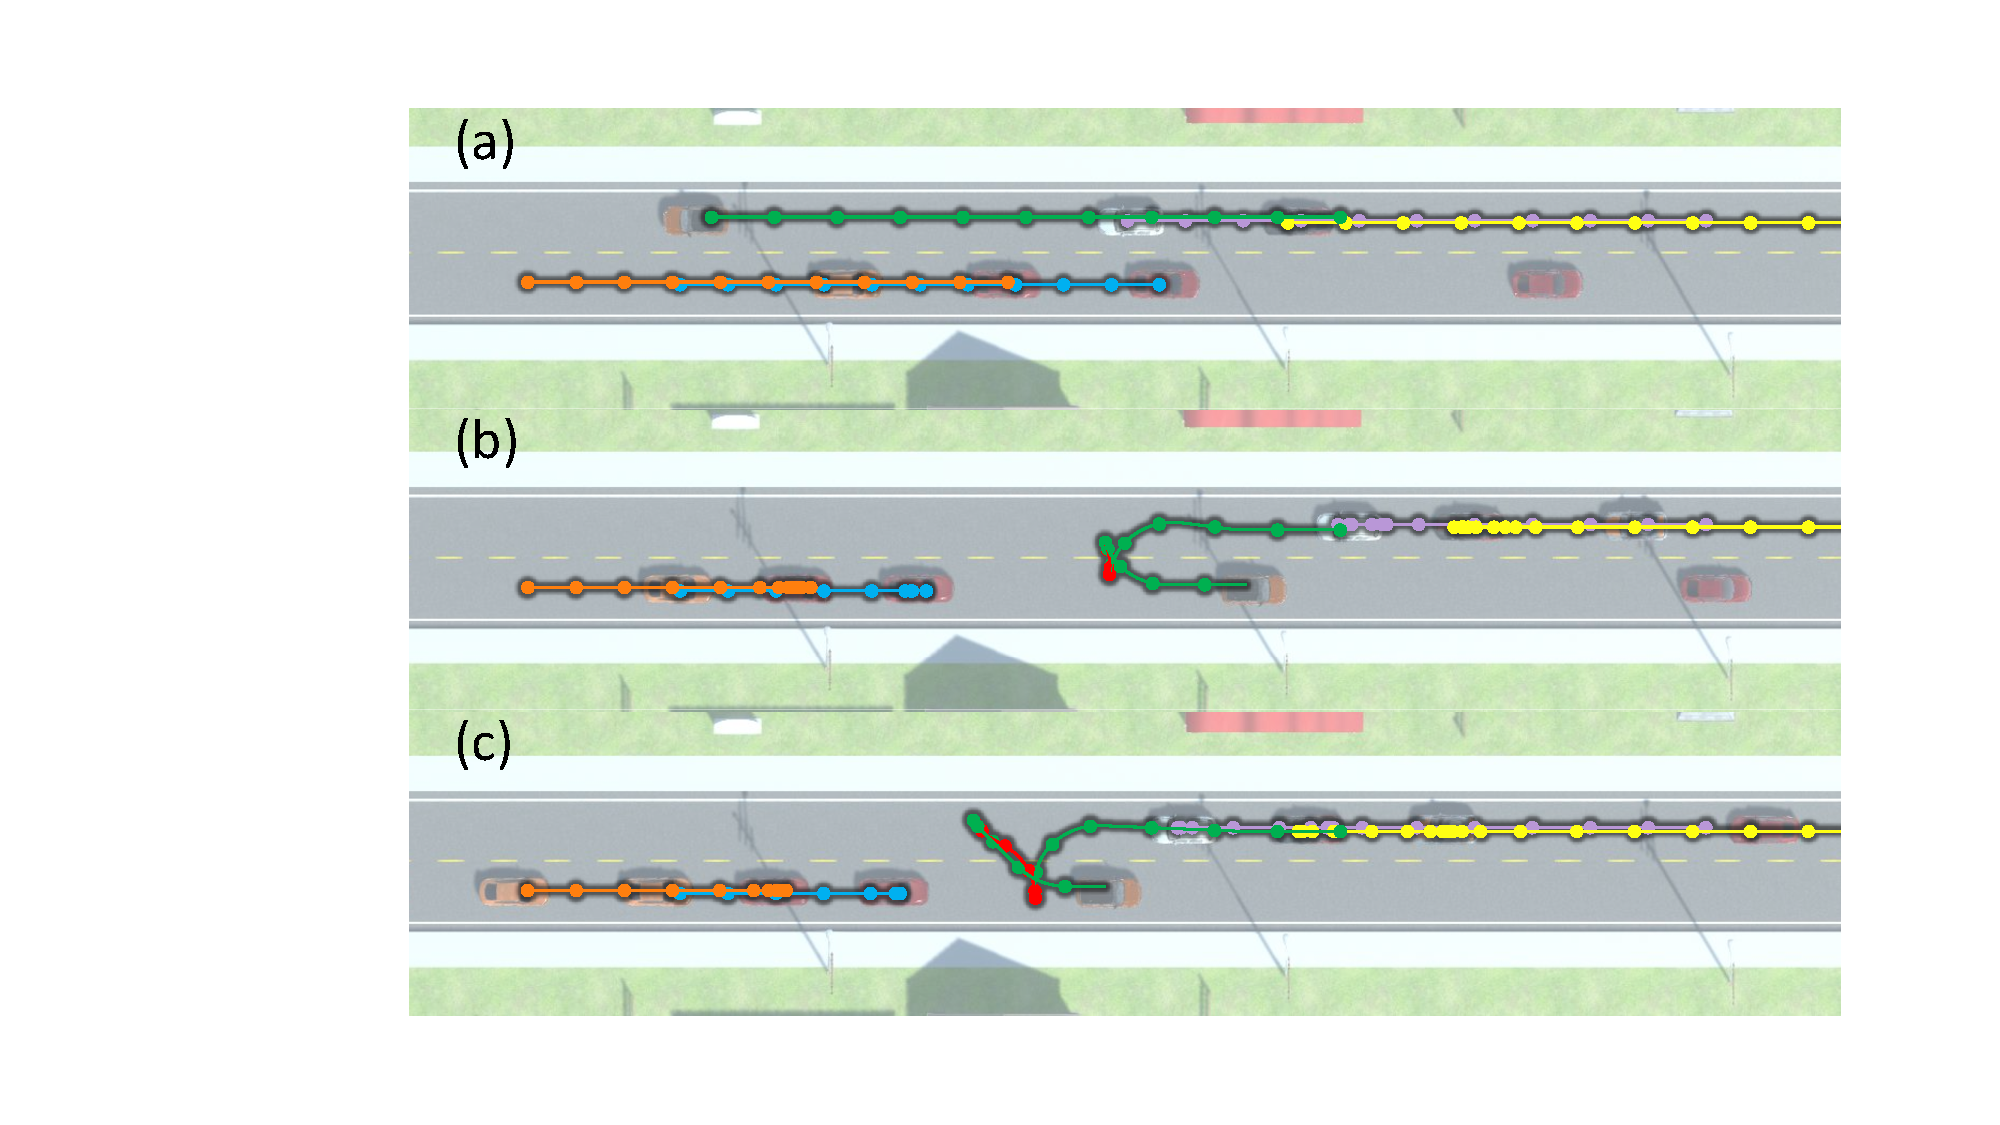
\includegraphics[width=0.9\textwidth]{figure/reversing/kturn v3.pdf}
%\caption[K型掉头编辑案例]{
%(a) 原始轨迹。(b,c) 被编辑车辆在空间有限的直道内K型掉头,用户可使用不同的输入控制倒车的距离。}
\caption[K型掉头编辑案例]{
K型掉头编辑案例
}
\label{fig:reversing_kturn}
\end{figure}

第一个案例在包含一条双向两车道的直道场景中生成,车道之间由黄色虚线分割,代表行驶中的车辆允许在借道、掉头等情况下越线进入对向车道。起初,被编辑车辆沿着其原本的车道自右往左行驶,如图~\ref{fig:reversing_kturn}(a)所示。我们使用一系列关键状态生成了一条新的参考路径,引导被编辑车辆进行K型掉头,如图~\ref{fig:reversing_kturn}(b)所示。K型掉头是在有限空间内让车辆调转方向行之有效的方式,需要驾驶员频繁在前进和倒车之间换挡。我们还可以微调生成参考路径所使用的关键状态,使被编辑车辆进行一段更长距离的倒车,如图~\ref{fig:reversing_kturn}(c)所示。最终,被编辑车辆成功在狭窄的道路上掉头并从另一条车道驶离场景。


第二个案例在包含十字路口的场景中生成,每一个路口为双向四车道。我们手动在特定的道路路口处放置了若干辆静止的车辆,用于模拟交通信号灯的控制。起初,被编辑车辆驶入被信号灯管控的车道,其同时被前车和后车堵塞,需要排队等待信号灯放行依次通过路口,如图~\ref{fig:reversing_escape}(a)所示。我们使用一系列关键状态生成了一条新的参考路径,引导其通过反复前进和后退获得更大的转向角,从侧方驶离被阻塞的队列,如图~\ref{fig:reversing_escape}(b)所示。最终,被编辑车辆从另一条车道通过了十字路口,而无需等待。

\begin{figure}[!tbh]
%\setlength{\abovecaptionskip}{-0.1cm} 
%\setlength{\belowcaptionskip}{-0.45cm}
\centering
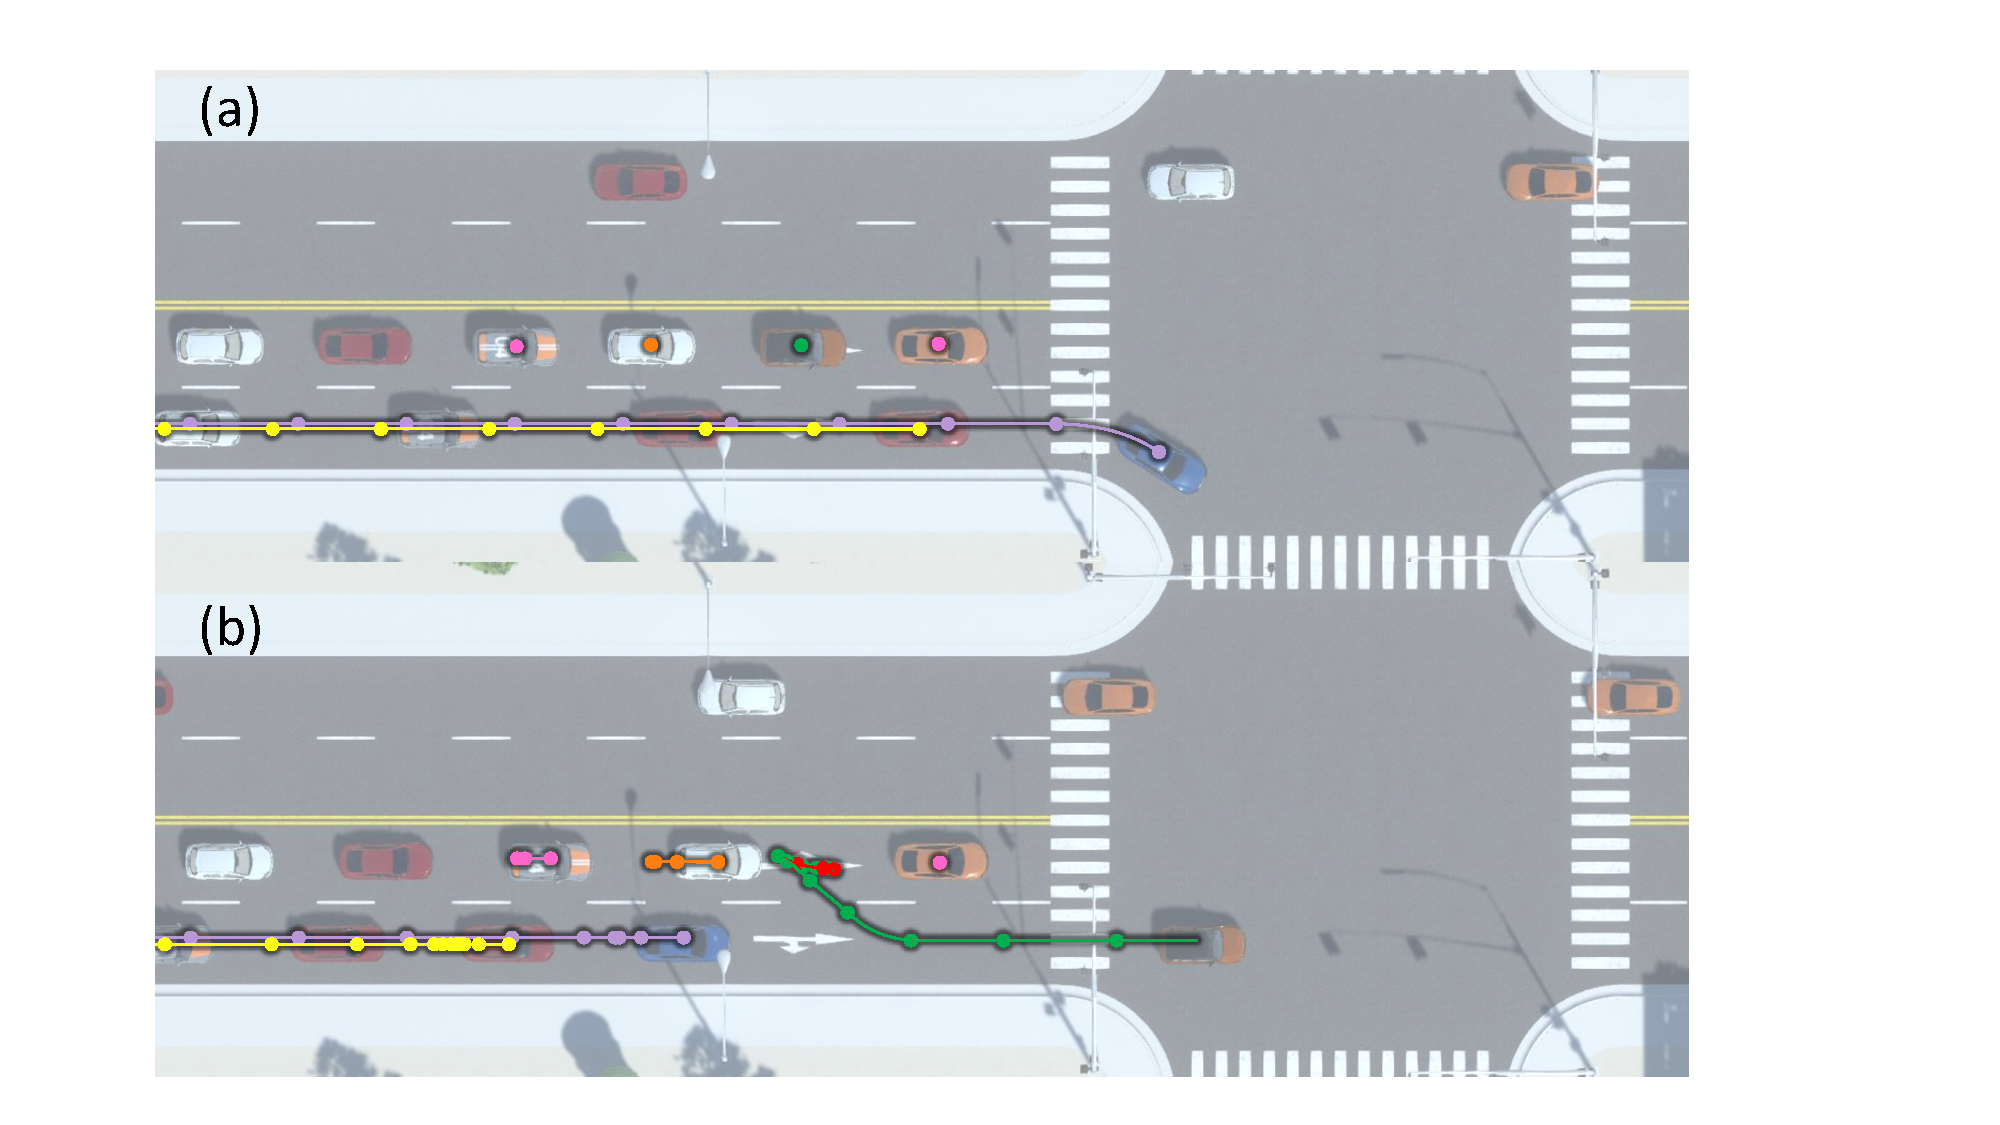
\includegraphics[width=0.9\textwidth]{figure/reversing/escape v3.pdf}
%\caption[侧方驶离编辑案例]{
%(a) 原始轨迹。(b) 被编辑车辆在前后均被堵塞的情况下通过侧方驶离并通过十字路口。}
\caption[侧方驶离编辑案例]{
侧方驶离编辑案例
}
\label{fig:reversing_escape}
\end{figure}


第三个案例在包含匝道的双向四车道公路场景中生成,所有的车道均非直线车道。起初,被编辑车辆在远离匝道口的车道上行驶,并没有考虑要离开主干道,如图~\ref{fig:reversing_ramp}(a)所示。我们使用一系列关键状态生成了一条新的参考路径,引导其在错过出口之后,通过倒车退回到匝道口,如图~\ref{fig:reversing_ramp}(b)所示。最终,被编辑车辆成功进入匝道,驶离了主干道。需要强调的是,该交通行为不符合交通规则,因此很少能被交通数据集捕捉,先前的仿真方法也鲜有考虑,但现实生活中仍然会因驾驶员的一时冲动偶尔发生。

\begin{figure}[!tbh]
%\setlength{\abovecaptionskip}{-0.1cm} 
%\setlength{\belowcaptionskip}{-0.45cm}
\centering
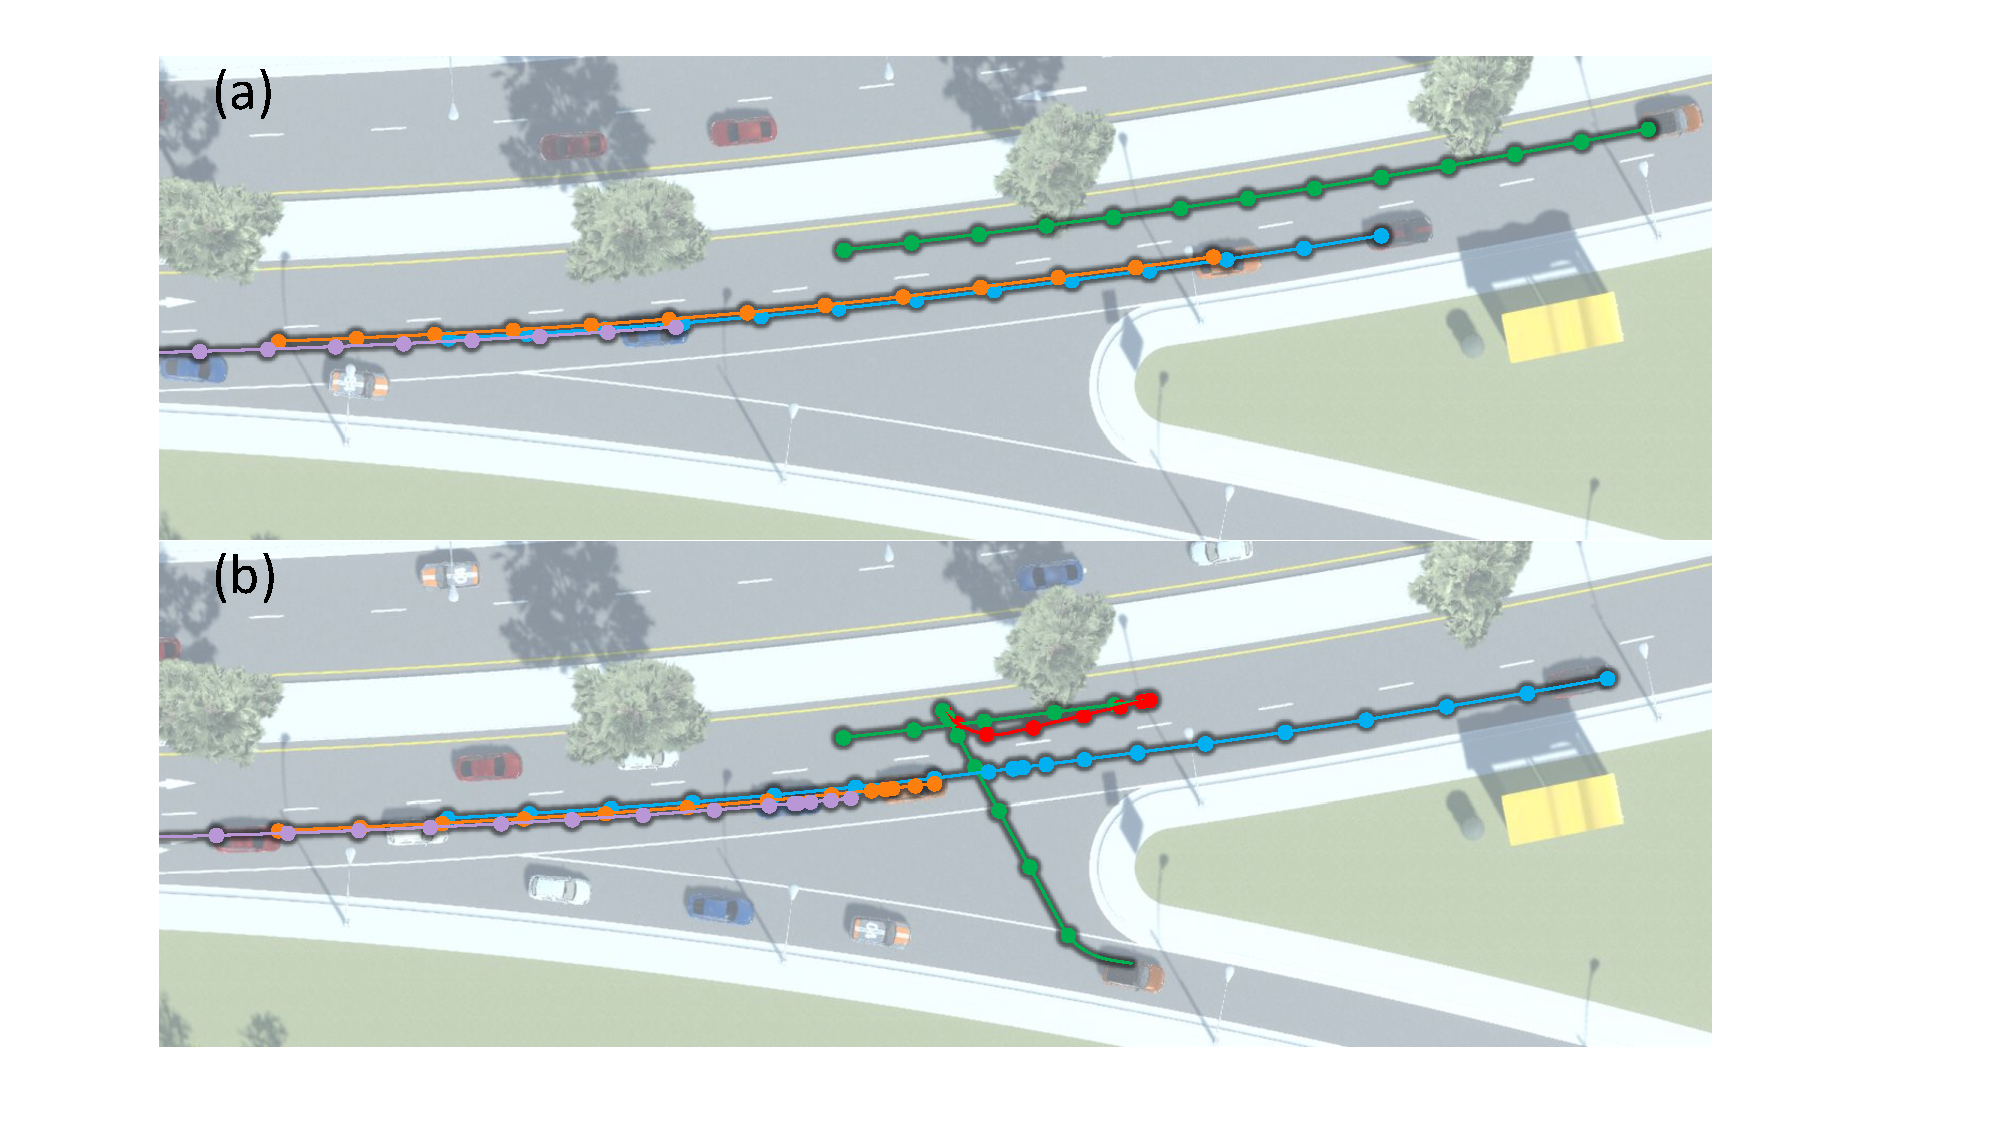
\includegraphics[width=0.9\textwidth]{figure/reversing/ramp v3.pdf}
%\caption[匝道口倒车编辑案例]{
%(a) 原始轨迹。(b) 被编辑车辆在错过匝道后倒车回到出口,最终从匝道离开。}
\caption[匝道口倒车编辑案例]{
匝道口倒车编辑案例
}
\label{fig:reversing_ramp}
\end{figure}


\subsection{对比实验}
\label{section:reversing_comparison}


基于上一节中自定义的带有反向导航的参考路径,我们对比了使用本方法生成的车辆运动与使用TraEDITS(章节~\ref{chapter:traedits})生成的车辆运动。如图~\ref{fig:reversing_orientcmp}所示,基于本方法仿真的车辆运动时朝向变化更平滑,这得益于我们为车辆状态更新的建模中引入了车辆的运动学模型(即表达式~\ref{eq:reversing_dynamics})。反观TraEDITS方法仿真的车辆,在参考路径导航方向切换的尖端点处车辆朝向会发生明显的突变,这是由于其在更新车辆状态时仅以参考路径为依据,而参考路径的方向在导航方向切换处并不连续。


\begin{figure}[!tbh]
%\setlength{\abovecaptionskip}{-0.1cm} 
%\setlength{\belowcaptionskip}{-0.45cm}
\centering
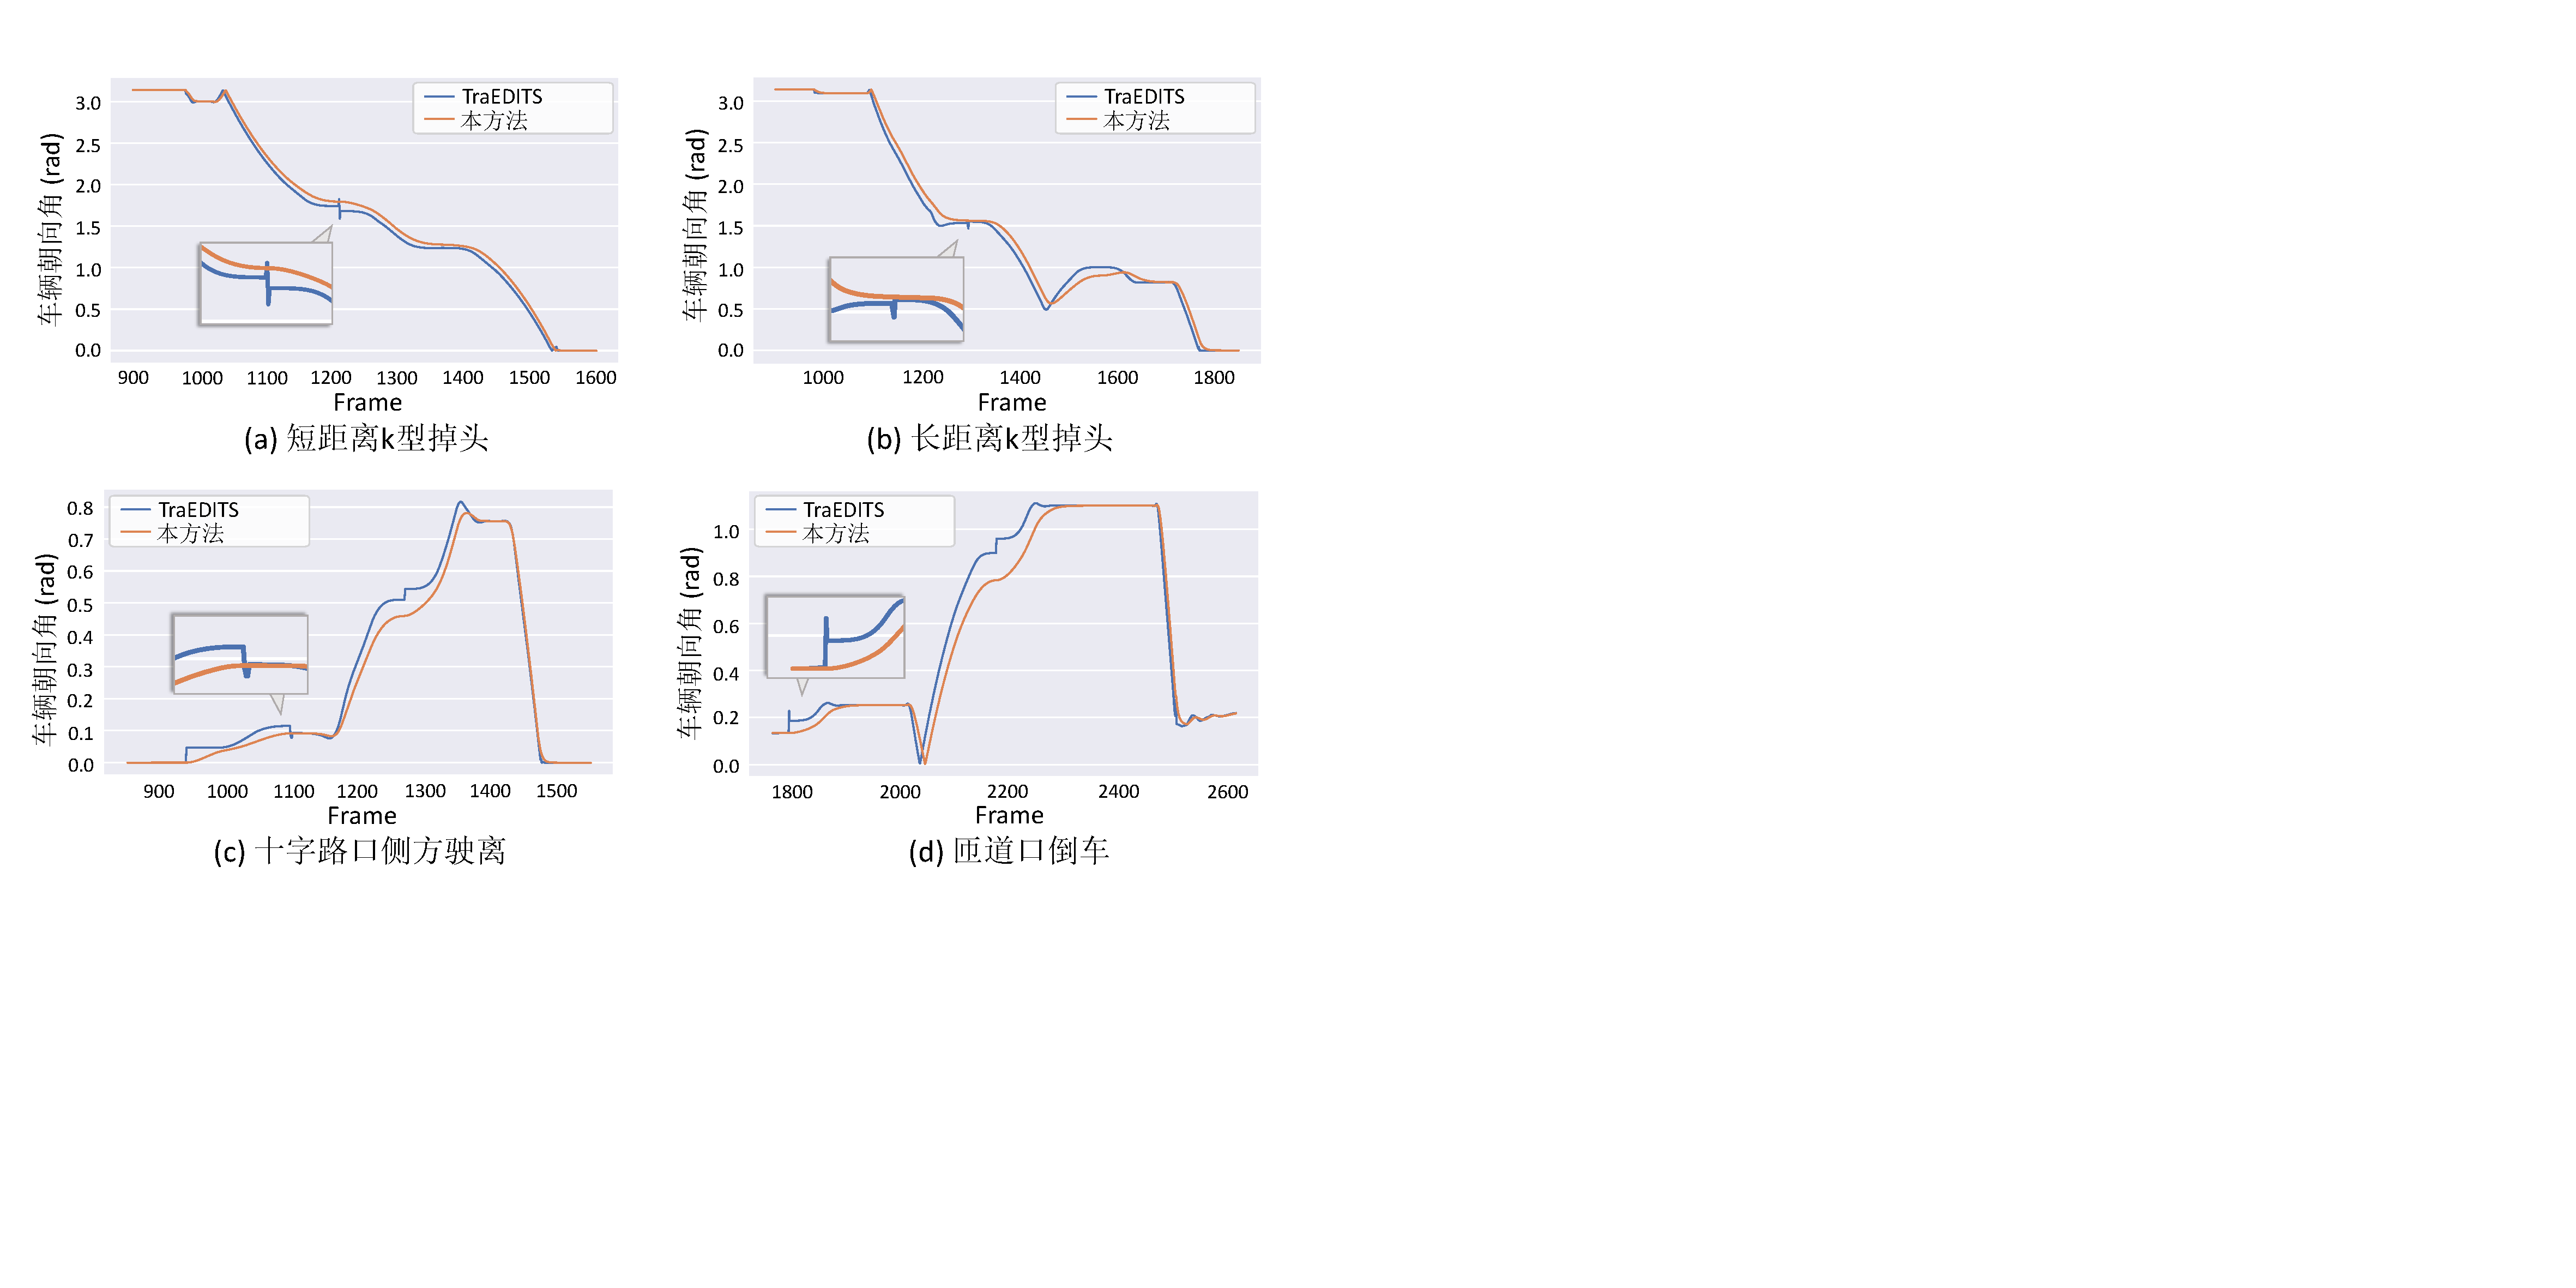
\includegraphics[width=0.95\textwidth]{figure/reversing/orientation v3.pdf}
%\caption[不同方法生成的车辆运动对比]{
%在跟随相同的参考路径时,使用本方法仿真的车辆运动与使用TraEDITS仿真的车辆运动,其朝向变化的对比曲线图。(a) 短距离倒车的K型掉头。(b) 长距离倒车的K型掉头。(c) 十字路口侧向驶离堵塞队列。(d) 错过出口倒车退回匝道口。}
\caption[不同方法生成的车辆方向变化对比]{
不同方法生成的车辆方向变化对比
}
\label{fig:reversing_orientcmp}
\end{figure}

我们设计了另一个实验案例:一辆车在其参考路径未来并未穿过静止的前车的情况下,跟随参考路径逐渐靠近前车,图~\ref{fig:reversing_heatmap}(f)中为该过程中某一时刻下的仿真截图。事实上,一辆车由于当前速度和转向角的限制,其特别在低速的时候是难以完美地跟随参考路径的导航的。因此,即使在路径规划过程中我们已经将静止的邻车视为障碍物,且生成的参考路径并不会导致碰撞,但车辆在实际行驶过程中仍有可能发生边缘剐蹭。为了展示本方法可以应对该情况,我们统计并绘制了更新车辆的能量最优化过程中各个能量项的热力图,而对应图~\ref{fig:reversing_heatmap}(f)结果时刻的能量热力图展示在(a)至(e)中。其中(a)代表可行域内的自驱动能量分布,(b)代表可行域内路径保持能量分布,(c)代表可行域内碰撞避免边界硬约束能量分布,(d)代表可行域内除边界硬约束能量外其余能量总和的分布,(e)代表可行域内所有能量总和的分布。特别地,我们将碰撞避免硬约束能量的数值进行了缩放,使其在数值上与接近其他能量项,便于热力图的可视化。基于表~\ref{tab:reversing_rules}中定义的交互规则,车辆跟随带有反向导航的参考路径时被视为非跟驰运动中,且参考路径未来并未穿过前车,所以安全跟随距离的约束在此时对于该车并未生效。因此,当不考虑碰撞避免硬约束时(图~\ref{fig:reversing_heatmap}(d)),车辆由于自驱动的作用会持续加速,最终导致在左前方与前车发生了轻微的剐蹭(图~\ref{fig:reversing_heatmap}(f)上);当考虑碰撞避免硬约束时(图~\ref{fig:reversing_heatmap}(e)),可行域内会发生剐蹭的候选速度会被限制在边界之外,此时车辆会在发生剐蹭之前减速并停止(图~\ref{fig:reversing_heatmap}(f)下)。为了在实际编辑过程中发生诸如此类的问题,用户可以迭代式地指定或者调整生成参考路径的关键状态。



\begin{figure}[!tbh]
%\setlength{\abovecaptionskip}{-0.1cm} 
%\setlength{\belowcaptionskip}{-0.45cm}
\centering
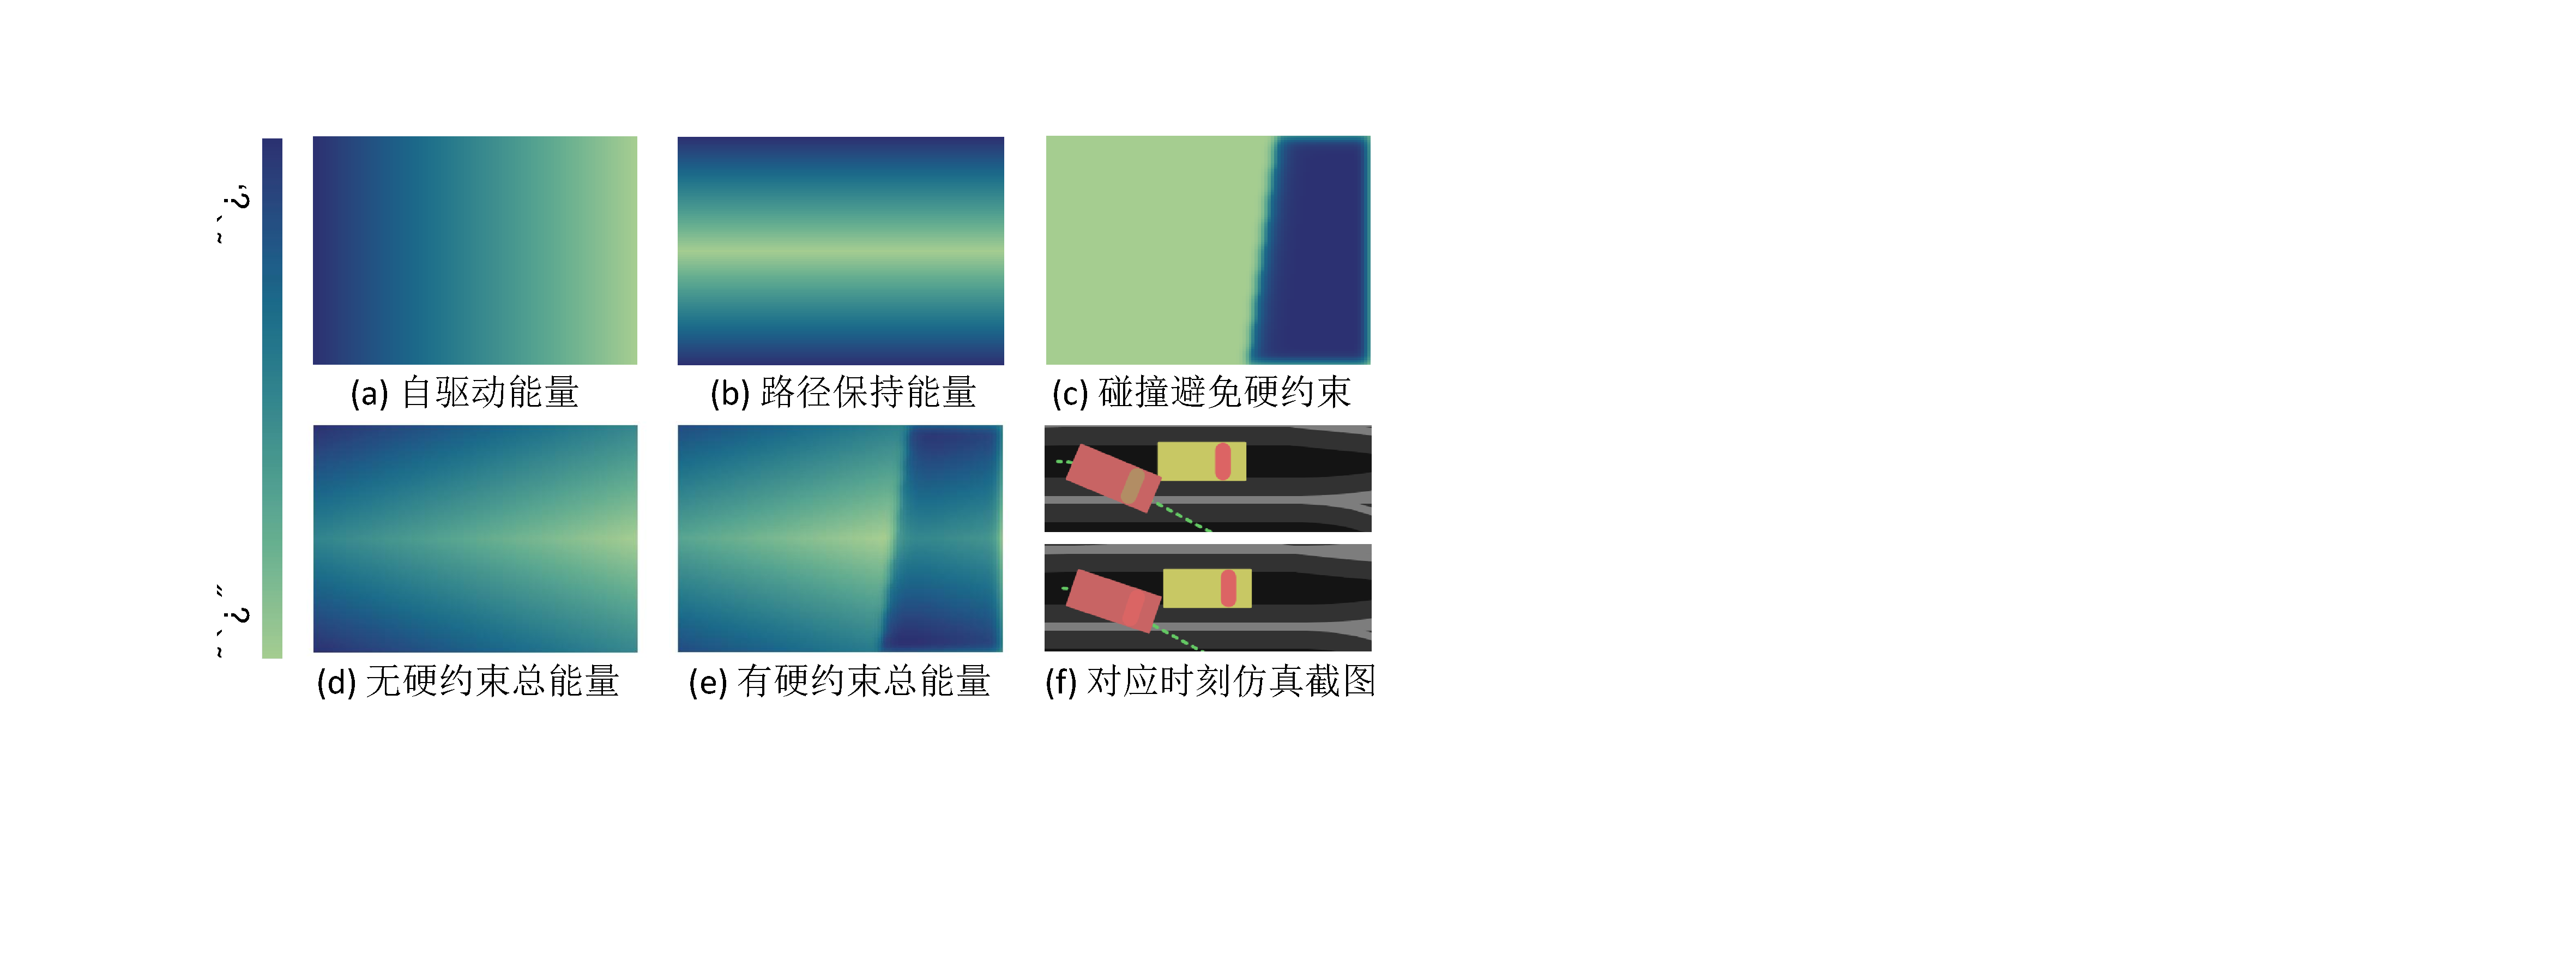
\includegraphics[width=0.8\textwidth]{figure/reversing/heatmap v4.pdf}
%\caption[能量最优化中各能量项的热力图]{
%车辆跟随参考路径靠近静止的前车,在某一时刻下更新车辆状态的能量最优化过程中各能量项的热力图。(a) 可行域内自驱动能量分布。(b) 可行域内路径保持能量分布。(c) 可行域内碰撞避免硬边界约束能量分布。(d) 可行域内,不带碰撞避免硬边界约束能量的总能量分布。(e) 可行域内,带碰撞避免硬边界约束的总能量分布。(f) 对应时刻的仿真截图,上、下图分别对应不带碰撞避免边界硬约束与带该约束的结果。}
\caption[能量最优化中各能量项的热力图]{
能量最优化中各能量项的热力图
}
\label{fig:reversing_heatmap}
\end{figure}


\subsection{用户调查}
\label{section:reversing_userstudy}

我们设计了一个用户调查以评估本方法是否能有效提高交互式轨迹编辑的可控程度和生成数据的多样性与非常规性。用户调查共有32位参与者,其中包含22位男性与10位女性,平均年龄为26.312岁。参与者被要求使用7分制的李克特量表回答一份调查问卷,打分的结果如图~\ref{fig:reversing_userstudy}所示,此外我们还对每一个问题通过假设其得分均高于中间数4分进行了单样本t检验。


\begin{figure}[!tbh]
%\setlength{\abovecaptionskip}{-0.1cm} 
%\setlength{\belowcaptionskip}{-0.45cm}
\centering
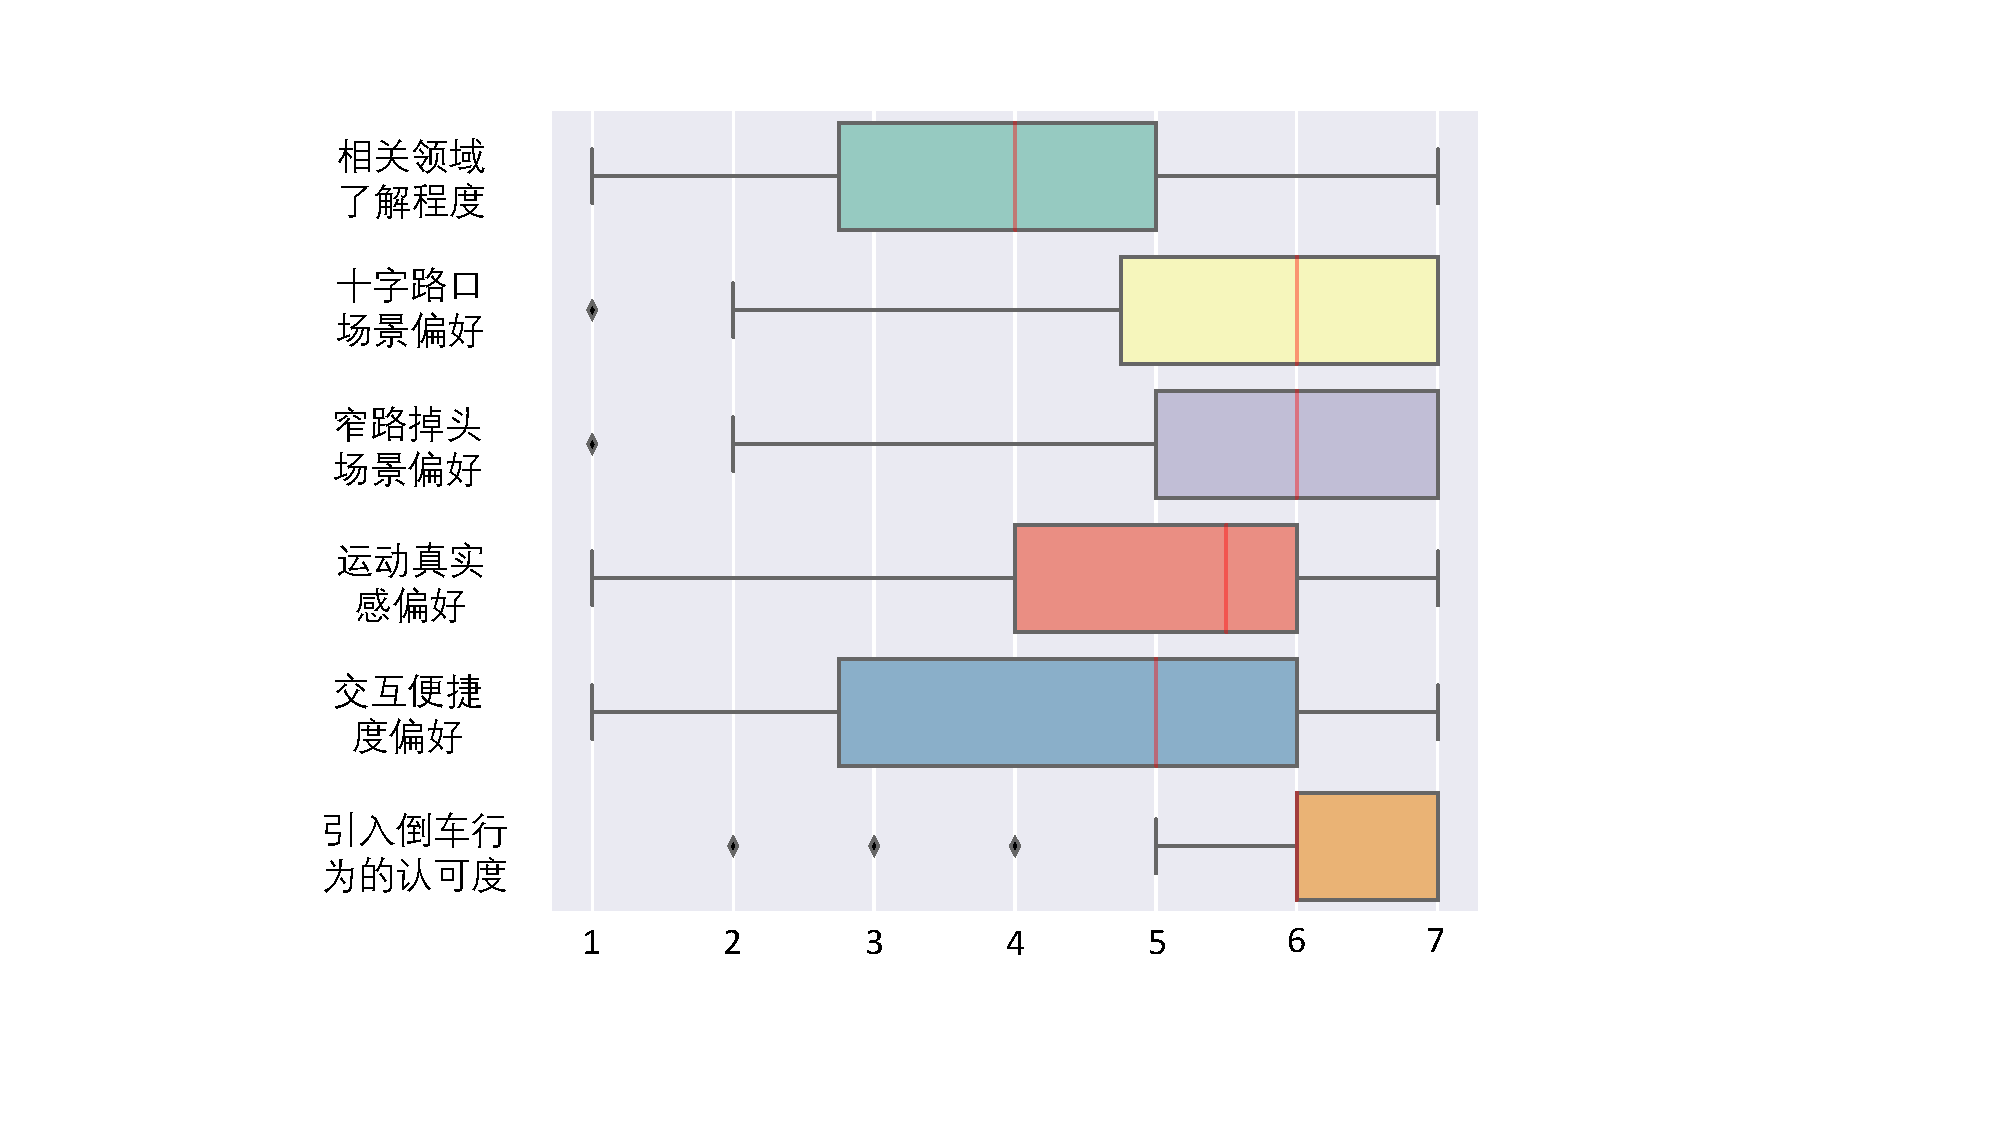
\includegraphics[width=0.75\textwidth]{figure/reversing/user study cn.pdf}
%\caption[用户调查的得分统计结果]{
%用户调查的得分统计结果,参与调查的人员被要求使用7分制的李克特量表对如下问题进行打分:在自动驾驶和交通仿真领域的知识储备量,对使用TraEDITS(1分)和本方法(7分)在不同场景中生成的结果偏好,对TraEDITS(1分)和本方法(7分)使用的交互编辑方式的偏好,以及是否赞同引入倒车行为能够提高生成轨迹数据和交通场景的多样性。}
\caption[用户调查的得分统计结果]{
用户调查的得分统计结果
}
\label{fig:reversing_userstudy}
\end{figure}

第一个问题中,我们询问了参与者在自动驾驶和交通仿真领域的储备量,其中1分代表毫无了解,7分代表十分精通。该题的得分表明了用户调查的参与者能覆盖自动驾驶和交通仿真领域的非专业人员和专家(均值$=3.843, t(32)=-0.487, p=0.630>0.05$)。

第二、第三个问题中,我们基于录制的视频,询问了参与者对使用不同方法进行轨迹编辑的结果偏好,其中1分代表更倾向于TraEDITS的轨迹编辑结果,7分代表更倾向于本方法的轨迹编辑结果。在第二个问题中的视频中,我们在十字路口的场景中通过编辑生成了侧向驶离堵塞队列的行为。该题的得分表明了本方法生成的结果显著受参与者的认可(均值$=5.438, t(32)=4.576, p \ll 0.001$),而TraEDITS生成的结果存在不真实的侧向漂移,违反了车辆的运动模式。在第三个问题的视频中,我们在狭窄的直道场景中通过编辑生成了掉头行为。该题的得分同样表明了本方法生成的结果显著受参与者的认可(均值$=5.563, t(32)=4.823, p \ll 0.001$),这是由于本方法可以生成更符合驾驶员习惯的K型掉头,而TraEDITS只能生成U型掉头,车辆在跟随其参考路径时即使考虑了减速和横向偏移的约束也缺乏真实感。

第四个问题中,我们基于录制的视频,询问了参与者对不同的方法驱动车辆跟随参考路径运动的真实感,参考路径同时包含前向和反向导航,其中1分代表更倾向于TraEDITS生成的车辆运动,7分代表更倾向于本方法生成的车辆运动。该题的得分表明了本方法生成的车辆运动在视觉上要显著平滑、连续(均值$=5.094, t(32)=3.742, p<0.001$)。


第五个问题中,我们询问了参与者对不同方法所使用的交互编辑方式的偏好,其中1分代表认为TraEDITS中点击关键位置点的形式更便捷,7分代表认为本方法中拖拽关键状态的形式更便捷。该题的得分表明了拖拽关键状态的形式与点击关键位置点的形式一样便捷(均值$=4.625, t(32)=1.743, p=0.091>0.05$),而拖拽关键点却能够包含更多的信息去生成带有反向导航的参考路径。

最后一个问题中,我们询问了参与者是否赞同引入倒车行为能够提高生成轨迹数据和交通场景的多样性,其中1分代表完全不同意,7分代表非常同意。该题的得分表明了参与者显著认可这一结论(均值$=6.094, t(32)=9.861, p \ll 
 0.001$)。



\section{本章小结}

本章提出了一个交互式交通仿真和编辑框架,通过在仿真过程中直观地拖拽一系列关键状态来引入倒车行为,生成具有跟驰和非跟驰运动的定制化交通轨迹。在给定的关键状态下,使用优化的混合A*算法,保证能够实时地生成具有前向和反向导航的新参考路径。然后在考虑了车辆运动学、自驱动、路径保持和碰撞避免的情况下,利用速度空间的采样和能量最优化更新车辆状态。通过设计多约束的碰撞避免能量项和制定特殊的交互规则,本方法可以保证沿着参考路径运动的车辆和邻车的反馈更平滑、真实,从而生成包含非常规行为的交通场景。由于整体个体运动控制策略借鉴了TrEDITS框架,因此本方法一样拥有实时的运行效率。

尽管目前结果暂时令人满意,但本方法仍然存在一些局限性。首先,在路径规划中并未充分利用车道信息,生成的参考路径以及跟随车辆可能偏离车道中心。即使该问题可以通过手动规划适当的参考路径来解决,发掘高效和鲁棒的路径规划算法也仍然是一个值得努力的方向。其次,我们的仿真方法和交互规则是基于经验建模的。在某些情况下,即使跟驰运动的来车有足够的时间先行通过,我们仍会强制其等待非跟驰运动中的邻车远离或结束运动,这也有悖于日常驾驶习惯(来自用户调查的反馈)。如何利用真实交通数据以进一步提高仿真结果的质量和可靠度,也仍然是一个挑战。


